% Options for packages loaded elsewhere
\PassOptionsToPackage{unicode}{hyperref}
\PassOptionsToPackage{hyphens}{url}
\PassOptionsToPackage{dvipsnames,svgnames,x11names}{xcolor}
%
\documentclass[
  letterpaper,
  DIV=11,
  numbers=noendperiod,
  landscape]{scrartcl}

\usepackage{amsmath,amssymb}
\usepackage{lmodern}
\usepackage{iftex}
\ifPDFTeX
  \usepackage[T1]{fontenc}
  \usepackage[utf8]{inputenc}
  \usepackage{textcomp} % provide euro and other symbols
\else % if luatex or xetex
  \usepackage{unicode-math}
  \defaultfontfeatures{Scale=MatchLowercase}
  \defaultfontfeatures[\rmfamily]{Ligatures=TeX,Scale=1}
\fi
% Use upquote if available, for straight quotes in verbatim environments
\IfFileExists{upquote.sty}{\usepackage{upquote}}{}
\IfFileExists{microtype.sty}{% use microtype if available
  \usepackage[]{microtype}
  \UseMicrotypeSet[protrusion]{basicmath} % disable protrusion for tt fonts
}{}
\makeatletter
\@ifundefined{KOMAClassName}{% if non-KOMA class
  \IfFileExists{parskip.sty}{%
    \usepackage{parskip}
  }{% else
    \setlength{\parindent}{0pt}
    \setlength{\parskip}{6pt plus 2pt minus 1pt}}
}{% if KOMA class
  \KOMAoptions{parskip=half}}
\makeatother
\usepackage{xcolor}
\setlength{\emergencystretch}{3em} % prevent overfull lines
\setcounter{secnumdepth}{-\maxdimen} % remove section numbering
% Make \paragraph and \subparagraph free-standing
\ifx\paragraph\undefined\else
  \let\oldparagraph\paragraph
  \renewcommand{\paragraph}[1]{\oldparagraph{#1}\mbox{}}
\fi
\ifx\subparagraph\undefined\else
  \let\oldsubparagraph\subparagraph
  \renewcommand{\subparagraph}[1]{\oldsubparagraph{#1}\mbox{}}
\fi

\usepackage{color}
\usepackage{fancyvrb}
\newcommand{\VerbBar}{|}
\newcommand{\VERB}{\Verb[commandchars=\\\{\}]}
\DefineVerbatimEnvironment{Highlighting}{Verbatim}{commandchars=\\\{\}}
% Add ',fontsize=\small' for more characters per line
\usepackage{framed}
\definecolor{shadecolor}{RGB}{241,243,245}
\newenvironment{Shaded}{\begin{snugshade}}{\end{snugshade}}
\newcommand{\AlertTok}[1]{\textcolor[rgb]{0.68,0.00,0.00}{#1}}
\newcommand{\AnnotationTok}[1]{\textcolor[rgb]{0.37,0.37,0.37}{#1}}
\newcommand{\AttributeTok}[1]{\textcolor[rgb]{0.40,0.45,0.13}{#1}}
\newcommand{\BaseNTok}[1]{\textcolor[rgb]{0.68,0.00,0.00}{#1}}
\newcommand{\BuiltInTok}[1]{\textcolor[rgb]{0.00,0.23,0.31}{#1}}
\newcommand{\CharTok}[1]{\textcolor[rgb]{0.13,0.47,0.30}{#1}}
\newcommand{\CommentTok}[1]{\textcolor[rgb]{0.37,0.37,0.37}{#1}}
\newcommand{\CommentVarTok}[1]{\textcolor[rgb]{0.37,0.37,0.37}{\textit{#1}}}
\newcommand{\ConstantTok}[1]{\textcolor[rgb]{0.56,0.35,0.01}{#1}}
\newcommand{\ControlFlowTok}[1]{\textcolor[rgb]{0.00,0.23,0.31}{#1}}
\newcommand{\DataTypeTok}[1]{\textcolor[rgb]{0.68,0.00,0.00}{#1}}
\newcommand{\DecValTok}[1]{\textcolor[rgb]{0.68,0.00,0.00}{#1}}
\newcommand{\DocumentationTok}[1]{\textcolor[rgb]{0.37,0.37,0.37}{\textit{#1}}}
\newcommand{\ErrorTok}[1]{\textcolor[rgb]{0.68,0.00,0.00}{#1}}
\newcommand{\ExtensionTok}[1]{\textcolor[rgb]{0.00,0.23,0.31}{#1}}
\newcommand{\FloatTok}[1]{\textcolor[rgb]{0.68,0.00,0.00}{#1}}
\newcommand{\FunctionTok}[1]{\textcolor[rgb]{0.28,0.35,0.67}{#1}}
\newcommand{\ImportTok}[1]{\textcolor[rgb]{0.00,0.46,0.62}{#1}}
\newcommand{\InformationTok}[1]{\textcolor[rgb]{0.37,0.37,0.37}{#1}}
\newcommand{\KeywordTok}[1]{\textcolor[rgb]{0.00,0.23,0.31}{#1}}
\newcommand{\NormalTok}[1]{\textcolor[rgb]{0.00,0.23,0.31}{#1}}
\newcommand{\OperatorTok}[1]{\textcolor[rgb]{0.37,0.37,0.37}{#1}}
\newcommand{\OtherTok}[1]{\textcolor[rgb]{0.00,0.23,0.31}{#1}}
\newcommand{\PreprocessorTok}[1]{\textcolor[rgb]{0.68,0.00,0.00}{#1}}
\newcommand{\RegionMarkerTok}[1]{\textcolor[rgb]{0.00,0.23,0.31}{#1}}
\newcommand{\SpecialCharTok}[1]{\textcolor[rgb]{0.37,0.37,0.37}{#1}}
\newcommand{\SpecialStringTok}[1]{\textcolor[rgb]{0.13,0.47,0.30}{#1}}
\newcommand{\StringTok}[1]{\textcolor[rgb]{0.13,0.47,0.30}{#1}}
\newcommand{\VariableTok}[1]{\textcolor[rgb]{0.07,0.07,0.07}{#1}}
\newcommand{\VerbatimStringTok}[1]{\textcolor[rgb]{0.13,0.47,0.30}{#1}}
\newcommand{\WarningTok}[1]{\textcolor[rgb]{0.37,0.37,0.37}{\textit{#1}}}

\providecommand{\tightlist}{%
  \setlength{\itemsep}{0pt}\setlength{\parskip}{0pt}}\usepackage{longtable,booktabs,array}
\usepackage{calc} % for calculating minipage widths
% Correct order of tables after \paragraph or \subparagraph
\usepackage{etoolbox}
\makeatletter
\patchcmd\longtable{\par}{\if@noskipsec\mbox{}\fi\par}{}{}
\makeatother
% Allow footnotes in longtable head/foot
\IfFileExists{footnotehyper.sty}{\usepackage{footnotehyper}}{\usepackage{footnote}}
\makesavenoteenv{longtable}
\usepackage{graphicx}
\makeatletter
\def\maxwidth{\ifdim\Gin@nat@width>\linewidth\linewidth\else\Gin@nat@width\fi}
\def\maxheight{\ifdim\Gin@nat@height>\textheight\textheight\else\Gin@nat@height\fi}
\makeatother
% Scale images if necessary, so that they will not overflow the page
% margins by default, and it is still possible to overwrite the defaults
% using explicit options in \includegraphics[width, height, ...]{}
\setkeys{Gin}{width=\maxwidth,height=\maxheight,keepaspectratio}
% Set default figure placement to htbp
\makeatletter
\def\fps@figure{htbp}
\makeatother

\usepackage{booktabs}
\usepackage{longtable}
\usepackage{array}
\usepackage{multirow}
\usepackage{wrapfig}
\usepackage{float}
\usepackage{colortbl}
\usepackage{pdflscape}
\usepackage{tabu}
\usepackage{threeparttable}
\usepackage{threeparttablex}
\usepackage[normalem]{ulem}
\usepackage{makecell}
\usepackage{xcolor}
\KOMAoption{captions}{tableheading}
\makeatletter
\makeatother
\makeatletter
\makeatother
\makeatletter
\@ifpackageloaded{caption}{}{\usepackage{caption}}
\AtBeginDocument{%
\ifdefined\contentsname
  \renewcommand*\contentsname{Table of contents}
\else
  \newcommand\contentsname{Table of contents}
\fi
\ifdefined\listfigurename
  \renewcommand*\listfigurename{List of Figures}
\else
  \newcommand\listfigurename{List of Figures}
\fi
\ifdefined\listtablename
  \renewcommand*\listtablename{List of Tables}
\else
  \newcommand\listtablename{List of Tables}
\fi
\ifdefined\figurename
  \renewcommand*\figurename{Figure}
\else
  \newcommand\figurename{Figure}
\fi
\ifdefined\tablename
  \renewcommand*\tablename{Table}
\else
  \newcommand\tablename{Table}
\fi
}
\@ifpackageloaded{float}{}{\usepackage{float}}
\floatstyle{ruled}
\@ifundefined{c@chapter}{\newfloat{codelisting}{h}{lop}}{\newfloat{codelisting}{h}{lop}[chapter]}
\floatname{codelisting}{Listing}
\newcommand*\listoflistings{\listof{codelisting}{List of Listings}}
\makeatother
\makeatletter
\@ifpackageloaded{caption}{}{\usepackage{caption}}
\@ifpackageloaded{subcaption}{}{\usepackage{subcaption}}
\makeatother
\makeatletter
\@ifpackageloaded{tcolorbox}{}{\usepackage[many]{tcolorbox}}
\makeatother
\makeatletter
\@ifundefined{shadecolor}{\definecolor{shadecolor}{rgb}{.97, .97, .97}}
\makeatother
\makeatletter
\makeatother
\ifLuaTeX
  \usepackage{selnolig}  % disable illegal ligatures
\fi
\IfFileExists{bookmark.sty}{\usepackage{bookmark}}{\usepackage{hyperref}}
\IfFileExists{xurl.sty}{\usepackage{xurl}}{} % add URL line breaks if available
\urlstyle{same} % disable monospaced font for URLs
\hypersetup{
  pdftitle={R and RStudio},
  colorlinks=true,
  linkcolor={blue},
  filecolor={Maroon},
  citecolor={Blue},
  urlcolor={Blue},
  pdfcreator={LaTeX via pandoc}}

\title{R and RStudio}
\author{}
\date{}

\begin{document}
\maketitle
\ifdefined\Shaded\renewenvironment{Shaded}{\begin{tcolorbox}[borderline west={3pt}{0pt}{shadecolor}, enhanced, boxrule=0pt, breakable, interior hidden, sharp corners, frame hidden]}{\end{tcolorbox}}\fi

\hypertarget{r-statistical-computing-graphics}{%
\subsection{R Statistical Computing \&
Graphics}\label{r-statistical-computing-graphics}}

\begin{itemize}
\tightlist
\item
  Free open souce software
\item
  Available for Windows, Mac and Linux/Unix operating systems
\item
  Large community of developers
\item
  Many packages/libraries

  \begin{itemize}
  \item
    CRAN repository
  \item
    Bioconductor repository
  \end{itemize}
\end{itemize}

\hypertarget{download-and-install}{%
\subsection{Download and Install}\label{download-and-install}}

Download the latest stable release of R fromhttps://www.r-project.org,
latest version is 4.2.3

\begin{figure}

\begin{minipage}[t]{0.70\linewidth}

{\centering 

\raisebox{-\height}{

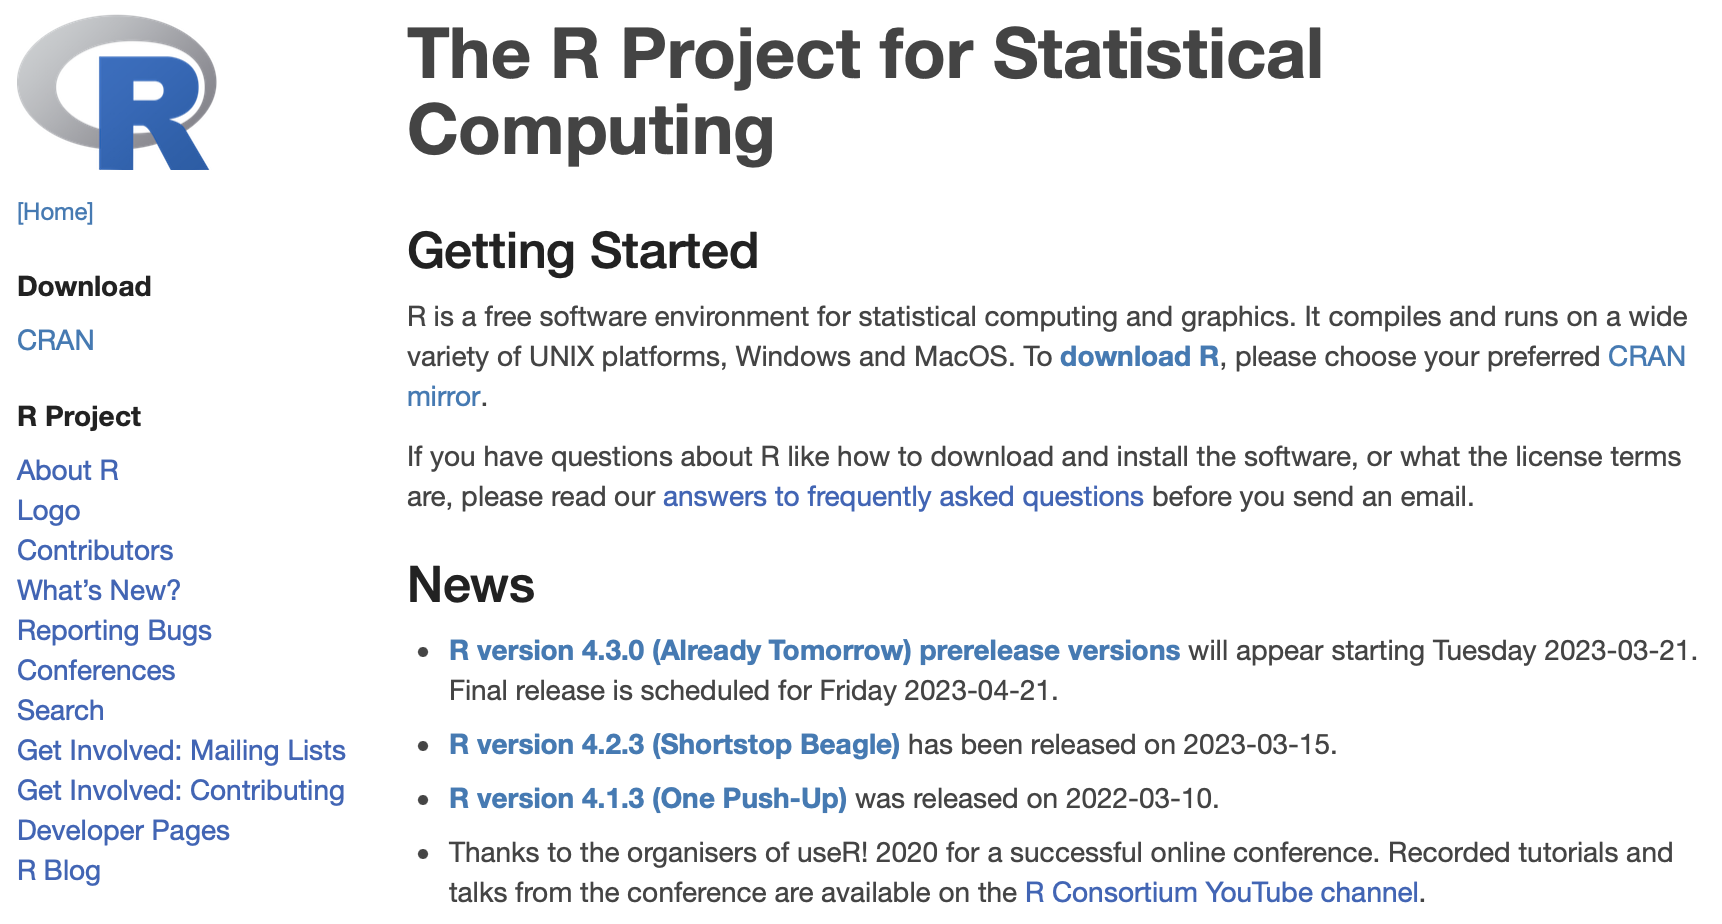
\includegraphics{images/R_home_screen.png}

}

}

\end{minipage}%
%
\begin{minipage}[t]{0.30\linewidth}

{\centering 

\raisebox{-\height}{

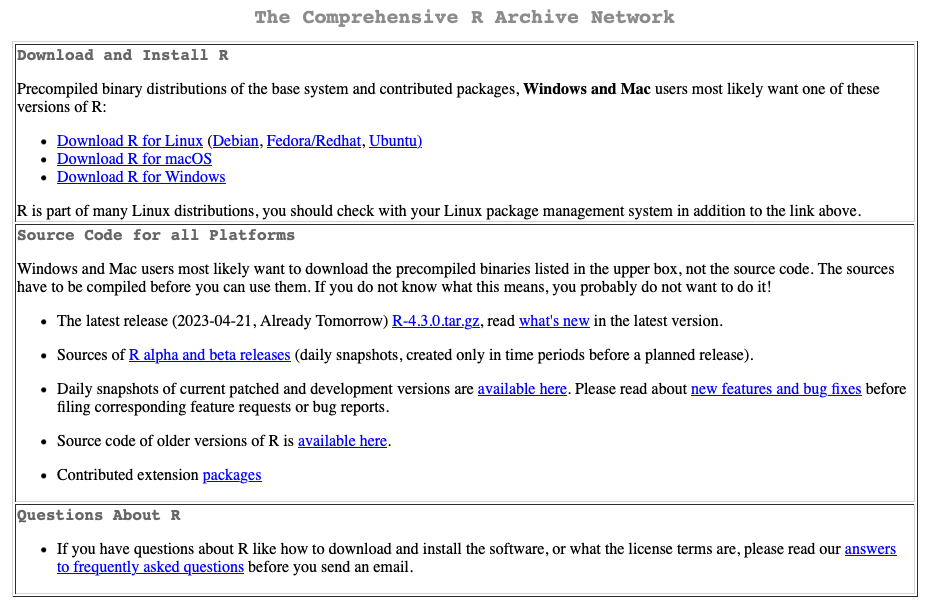
\includegraphics{images/R_download_versions.png}

}

}

\end{minipage}%

\end{figure}

\hypertarget{rstudio}{%
\subsection{RStudio}\label{rstudio}}

\begin{itemize}
\tightlist
\item
  Integrated development environment (IDE)

  \begin{itemize}
  \tightlist
  \item
    R
  \item
    Python
  \end{itemize}
\item
  Console for running code
\item
  Code editor with syntax colouring
\item
  Workspace/file managment
\item
  Records history of commands
\end{itemize}

\hypertarget{rstudio-1}{%
\subsection{RStudio}\label{rstudio-1}}

Download from https://posit.co/download/rstudio-desktop/

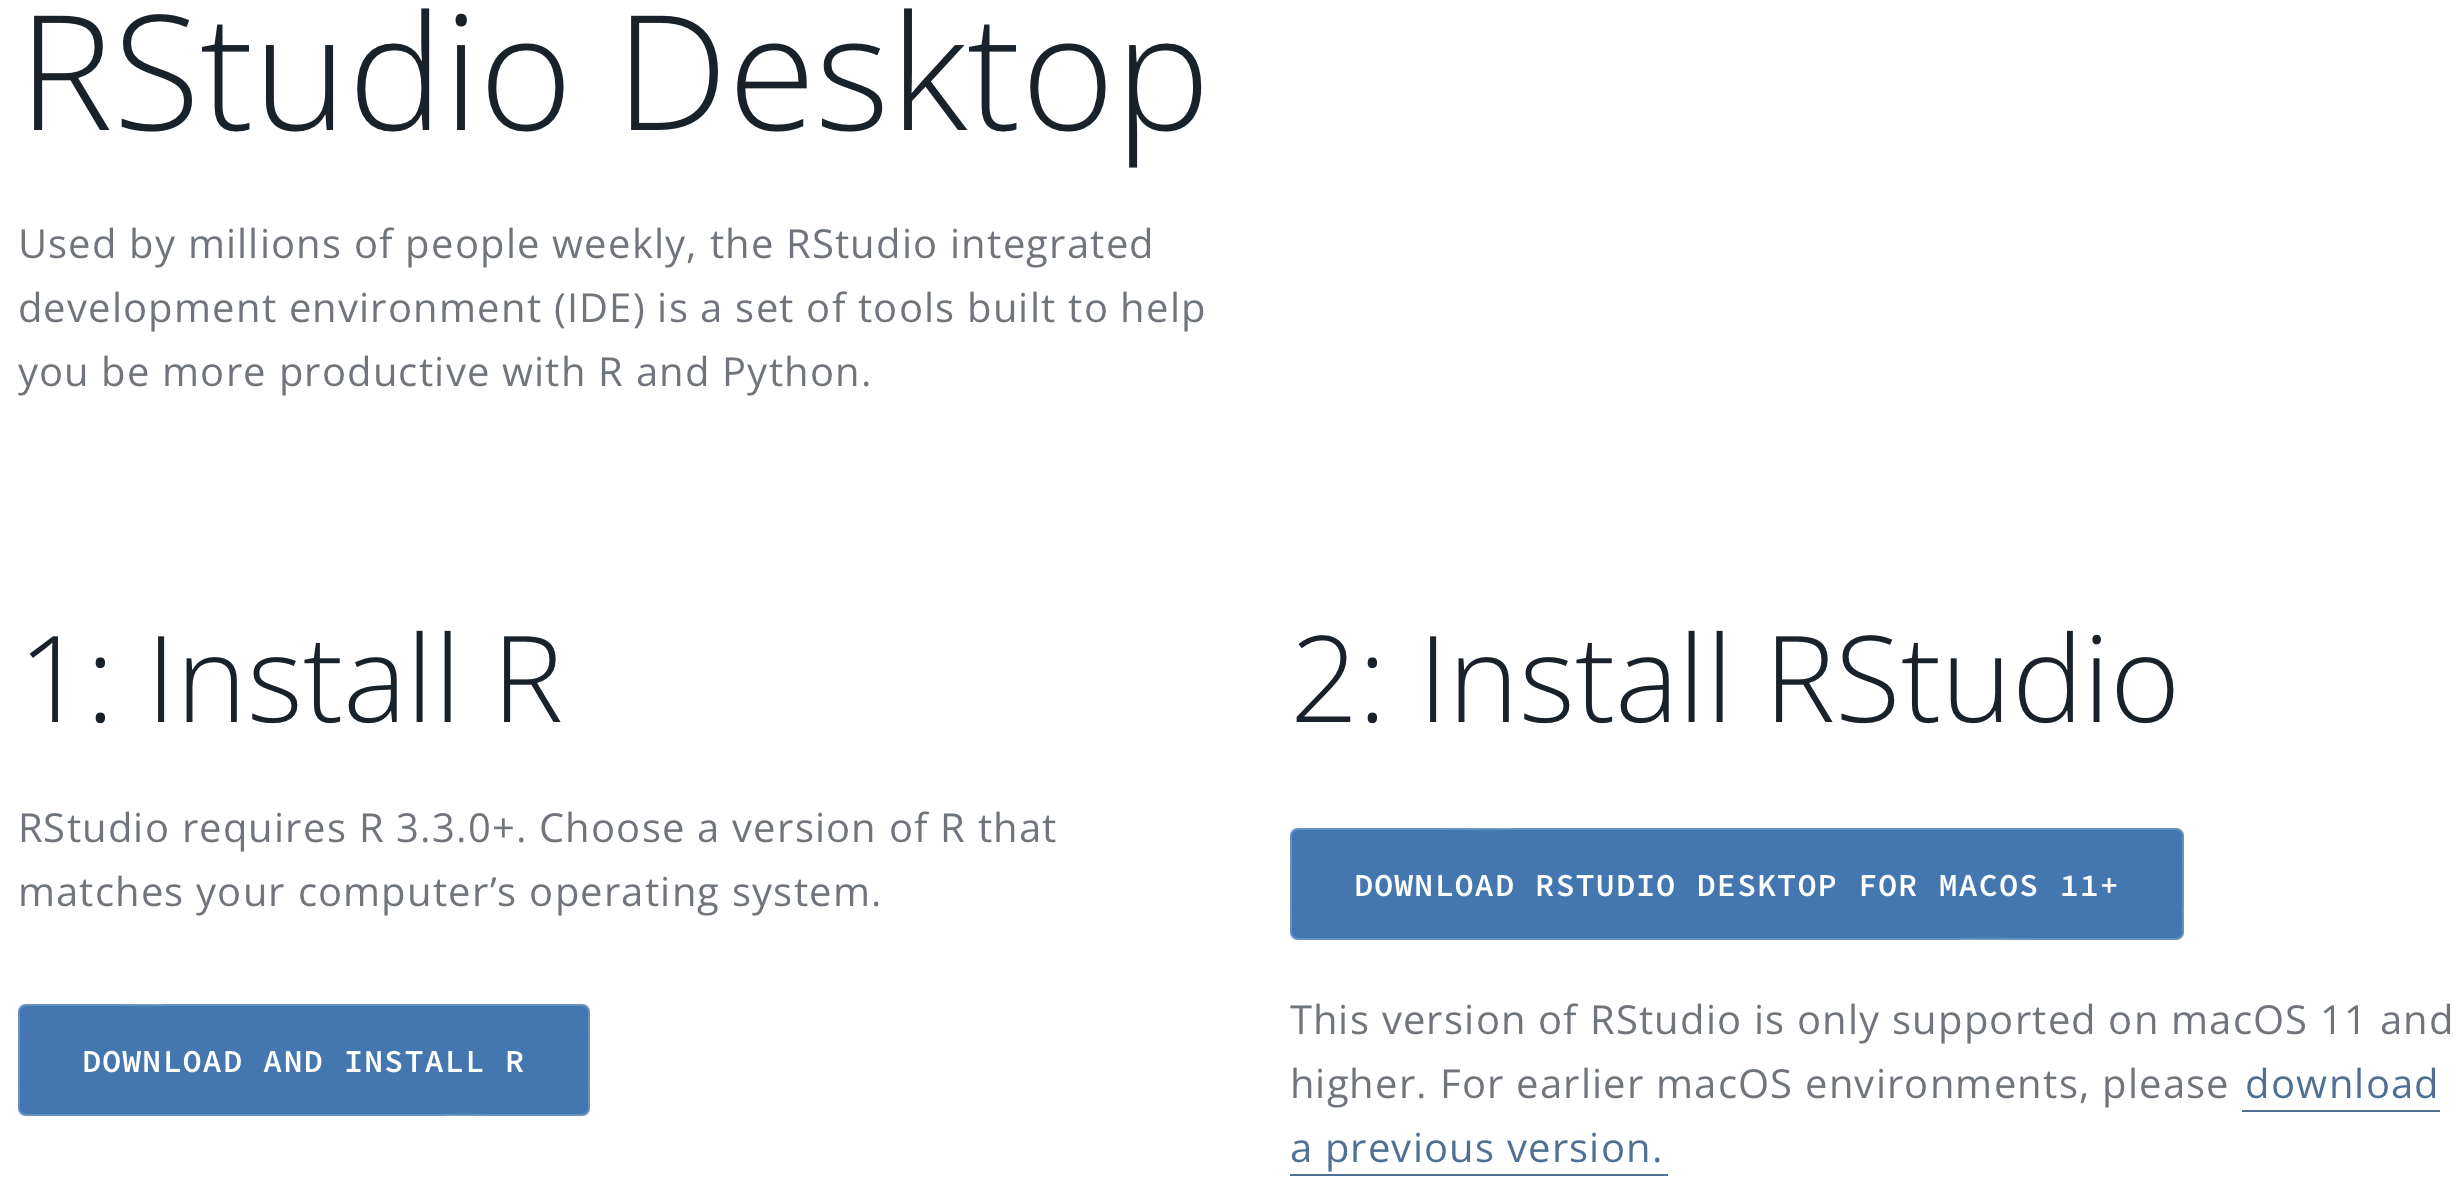
\includegraphics[width=1\textwidth,height=\textheight]{images/RStudio_download.png}

\begin{itemize}
\tightlist
\item
  This page should detect your operating system
\item
  Download RStudio
\item
  Click on the install package
\item
  Follow install instructions
\end{itemize}

\hypertarget{section}{%
\subsection{}\label{section}}

\hypertarget{rstudio-2}{%
\subsection{RStudio}\label{rstudio-2}}

Set up Rstudio - Set options in \textbf{Tools} and \textbf{Global
Options\ldots{}}

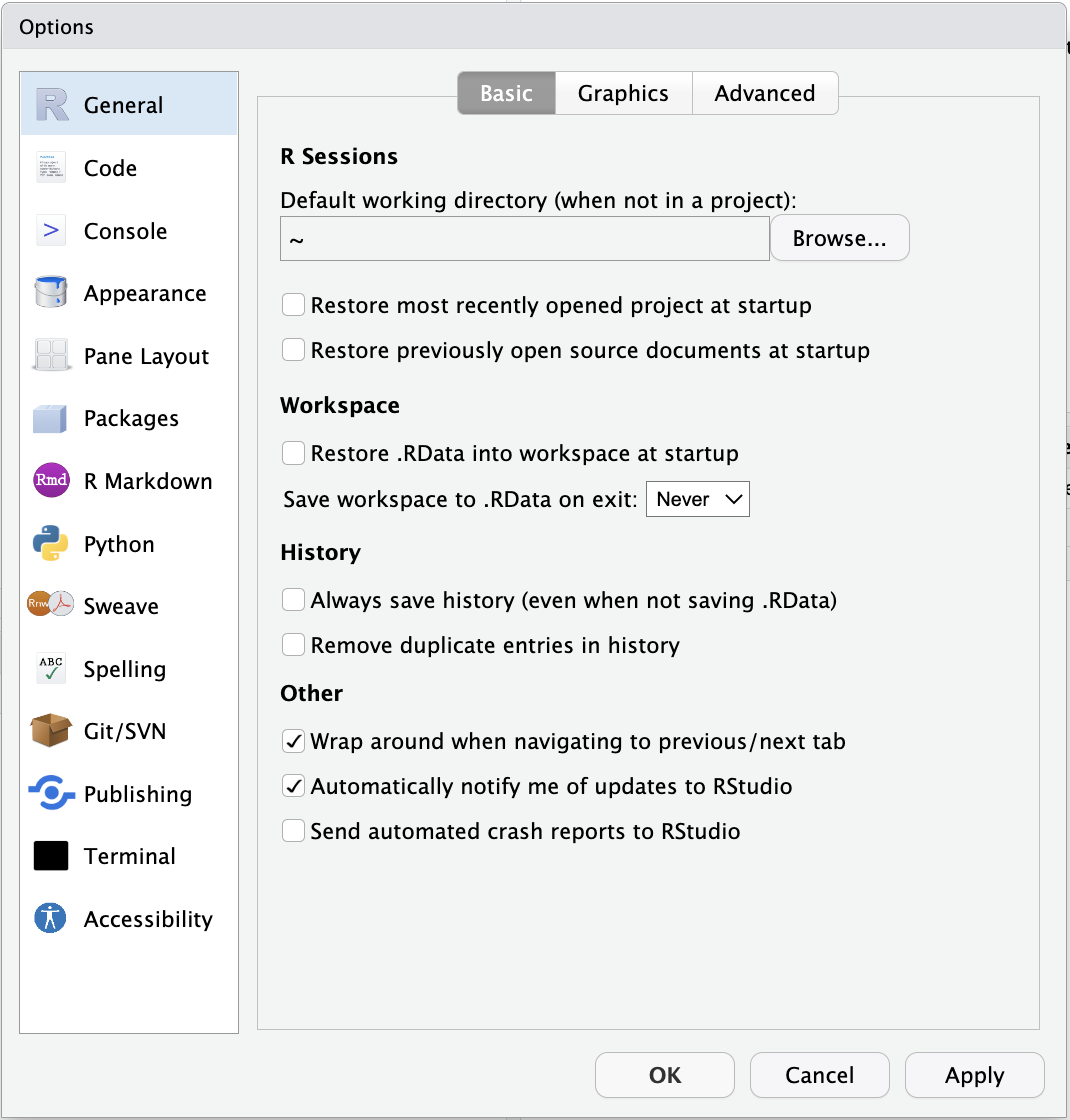
\includegraphics[width=1\textwidth,height=\textheight]{images/RStudio_settings.png}

\begin{itemize}
\tightlist
\item
  Uncheck the boxes as shown in the example
\item
  Ensure that \emph{Save workspace to .RData on exit} is set to
  \textbf{Never}
\end{itemize}

{YouTube video on installing and setting up RStudio
https://www.youtube.com/watch?v=D6CunpqF04E}

\hypertarget{rstudio-3}{%
\subsection{RStudio}\label{rstudio-3}}

\includegraphics[width=1\textwidth,height=\textheight]{images/RStudio_panels.png}

\begin{itemize}
\tightlist
\item
  {Source pane}

  \begin{itemize}
  \tightlist
  \item
    Write R commands as R scripts or Notebooks\\
  \end{itemize}
\item
  {Console Pane}

  \begin{itemize}
  \tightlist
  \item
    Where the R commands are executed
  \end{itemize}
\item
  {Environment pane}

  \begin{itemize}
  \tightlist
  \item
    Details of the R variables
  \end{itemize}
\item
  {Files pane}

  \begin{itemize}
  \tightlist
  \item
    View the directory and file structure
  \end{itemize}
\end{itemize}

\hypertarget{rstudio-libraries}{%
\subsection{RStudio Libraries}\label{rstudio-libraries}}

R packages or libraries are extensions to the R language.\\
R packages contain:

\begin{itemize}
\tightlist
\item
  Code\\
\item
  Data\\
\item
  Documentation
\end{itemize}

The packages are in a standardised format and can be installed from
repositories

\hypertarget{r-repositories}{%
\subsection{R Repositories}\label{r-repositories}}

\begin{itemize}
\tightlist
\item
  Comprehensive R Archive Network (CRAN)

  \begin{itemize}
  \tightlist
  \item
    Main software repositiry, supported by the R Foundation
  \end{itemize}
\item
  Bioconductor

  \begin{itemize}
  \tightlist
  \item
    R packages for the analysis of biological data
  \end{itemize}
\item
  GitHub

  \begin{itemize}
  \tightlist
  \item
    Alternative repository for R packages, often in active development
  \end{itemize}
\end{itemize}

\hypertarget{installing-libraries}{%
\subsection{Installing Libraries}\label{installing-libraries}}

\hypertarget{rstudio-4}{%
\subsubsection{RStudio}\label{rstudio-4}}

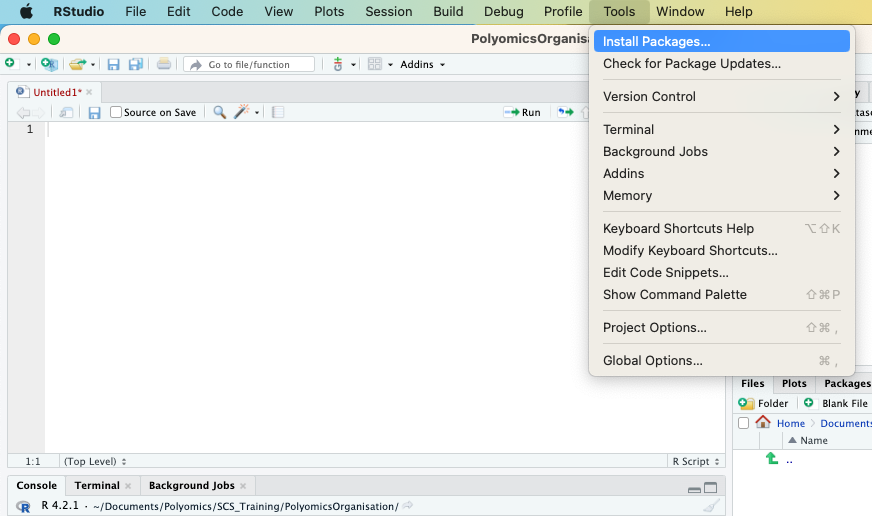
\includegraphics[width=\textwidth,height=5.20833in]{images/RStudio_tools.png}

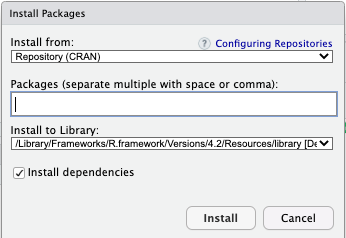
\includegraphics[width=3.60417in,height=2.47917in]{images/RStudio_package_installer.png}

\hypertarget{installing-packages}{%
\subsection{Installing Packages}\label{installing-packages}}

\hypertarget{terminal}{%
\subsubsection{Terminal}\label{terminal}}

From CRAN using the R command install.packages

\begin{Shaded}
\begin{Highlighting}[]
\FunctionTok{install.packages}\NormalTok{(}\StringTok{"tidyverse"}\NormalTok{)}
\end{Highlighting}
\end{Shaded}

From Bioconductor First need to install a package manager program

\begin{Shaded}
\begin{Highlighting}[]
\ControlFlowTok{if}\NormalTok{ (}\SpecialCharTok{!}\FunctionTok{require}\NormalTok{(}\StringTok{"BiocManager"}\NormalTok{, }\AttributeTok{quietly =} \ConstantTok{TRUE}\NormalTok{))}
    \FunctionTok{install.packages}\NormalTok{(}\StringTok{"BiocManager"}\NormalTok{)}
\NormalTok{BiocManager}\SpecialCharTok{::}\FunctionTok{install}\NormalTok{()}
\end{Highlighting}
\end{Shaded}

Then can install specific packages

\begin{Shaded}
\begin{Highlighting}[]
\NormalTok{BiocManager}\SpecialCharTok{::}\FunctionTok{install}\NormalTok{(}\FunctionTok{c}\NormalTok{(}\StringTok{"GenomicFeatures"}\NormalTok{, }\StringTok{"AnnotationDbi"}\NormalTok{))}
\end{Highlighting}
\end{Shaded}

\hypertarget{installing-packages-1}{%
\subsection{Installing Packages}\label{installing-packages-1}}

\hypertarget{terminal-1}{%
\subsubsection{Terminal}\label{terminal-1}}

From GitHub First need to install devtools from CRAN

\begin{Shaded}
\begin{Highlighting}[]
\FunctionTok{install.packages}\NormalTok{(}\StringTok{"devtools"}\NormalTok{)}
\FunctionTok{require}\NormalTok{(}\StringTok{"devtools"}\NormalTok{)}
\end{Highlighting}
\end{Shaded}

Then can install GitHub packages. Github packages are usually named
after the repository name then the package name
e.g.~grahamhamilton/Rpackage

\begin{Shaded}
\begin{Highlighting}[]
\FunctionTok{install\_github}\NormalTok{(}\StringTok{"GitHubPackage"}\NormalTok{)}
\end{Highlighting}
\end{Shaded}

\hypertarget{installing-packages-2}{%
\subsection{Installing Packages}\label{installing-packages-2}}

Now install these packages

\begin{itemize}
\item
  CRAN

  \begin{itemize}
  \item
    tidyverse
  \item
    devtools
  \end{itemize}
\end{itemize}

\hypertarget{section-1}{%
\subsection{}\label{section-1}}

\hypertarget{loading-packages}{%
\subsection{Loading Packages}\label{loading-packages}}

Packages have to be loaded prior to use. There are two ways to load
packages in R.

\begin{itemize}
\tightlist
\item
  \textbf{library()}

  \begin{itemize}
  \tightlist
  \item
    library() will output an error and stop the execution of the code
  \end{itemize}
\item
  \textbf{require()}

  \begin{itemize}
  \tightlist
  \item
    require() will output a warning if a package is not installed and
    then continue to execute the code
  \end{itemize}
\end{itemize}

\hypertarget{loading-packages-1}{%
\subsection{Loading Packages}\label{loading-packages-1}}

Load the libraries seperately

\begin{Shaded}
\begin{Highlighting}[]
\FunctionTok{library}\NormalTok{(}\StringTok{"tidyverse"}\NormalTok{)}
\end{Highlighting}
\end{Shaded}

\begin{verbatim}
-- Attaching core tidyverse packages ------------------------ tidyverse 2.0.0 --
v dplyr     1.1.0     v readr     2.1.4
v forcats   1.0.0     v stringr   1.5.0
v ggplot2   3.4.2     v tibble    3.2.1
v lubridate 1.9.2     v tidyr     1.3.0
v purrr     1.0.1     
-- Conflicts ------------------------------------------ tidyverse_conflicts() --
x dplyr::filter() masks stats::filter()
x dplyr::lag()    masks stats::lag()
i Use the ]8;;http://conflicted.r-lib.org/conflicted package]8;; to force all conflicts to become errors
\end{verbatim}

\begin{Shaded}
\begin{Highlighting}[]
\FunctionTok{library}\NormalTok{(}\StringTok{"Rsubread"}\NormalTok{)}
\end{Highlighting}
\end{Shaded}

Or as a comma seperated list

\begin{Shaded}
\begin{Highlighting}[]
\FunctionTok{library}\NormalTok{(}\StringTok{"tidyverse"}\NormalTok{,}\StringTok{"Rsubread"}\NormalTok{)}
\end{Highlighting}
\end{Shaded}

\hypertarget{loading-packages-2}{%
\subsection{Loading Packages}\label{loading-packages-2}}

Loading packages within a function from CRAN

\begin{Shaded}
\begin{Highlighting}[numbers=left,,]
\NormalTok{cran.packages }\OtherTok{\textless{}{-}} \FunctionTok{c}\NormalTok{(}\StringTok{"tidyverse"}\NormalTok{,}
                   \StringTok{"kableExtra"}\NormalTok{)}

\NormalTok{cran.load }\OtherTok{\textless{}{-}} \ControlFlowTok{function}\NormalTok{(pkg)\{}
\NormalTok{        new.pkg }\OtherTok{\textless{}{-}}\NormalTok{ pkg[}\SpecialCharTok{!}\NormalTok{(pkg }\SpecialCharTok{\%in\%} \FunctionTok{installed.packages}\NormalTok{()[, }\StringTok{"Package"}\NormalTok{])]}
        \ControlFlowTok{if}\NormalTok{ (}\FunctionTok{length}\NormalTok{(new.pkg))\{}
          \FunctionTok{install.packages}\NormalTok{(new.pkg, }\AttributeTok{dependencies =} \ConstantTok{TRUE}\NormalTok{)}
\NormalTok{          \}}
        \FunctionTok{sapply}\NormalTok{(pkg, require, }\AttributeTok{character.only =} \ConstantTok{TRUE}\NormalTok{)}
\NormalTok{\}}
\FunctionTok{cran.load}\NormalTok{(cran.packages)}
\end{Highlighting}
\end{Shaded}

\begin{verbatim}
Loading required package: kableExtra
\end{verbatim}

\begin{verbatim}

Attaching package: 'kableExtra'
\end{verbatim}

\begin{verbatim}
The following object is masked from 'package:dplyr':

    group_rows
\end{verbatim}

\begin{verbatim}
 tidyverse kableExtra 
      TRUE       TRUE 
\end{verbatim}

\hypertarget{loading-packages-3}{%
\subsection{Loading Packages}\label{loading-packages-3}}

Loading packages within a function from Bioconductor

\begin{Shaded}
\begin{Highlighting}[numbers=left,,]
\NormalTok{biomart.packages }\OtherTok{\textless{}{-}} \FunctionTok{c}\NormalTok{(}\StringTok{"Rsubread"}\NormalTok{)}

\NormalTok{biomart.load }\OtherTok{\textless{}{-}} \ControlFlowTok{function}\NormalTok{(pkg)\{}
\NormalTok{        new.pkg }\OtherTok{\textless{}{-}}\NormalTok{ pkg[}\SpecialCharTok{!}\NormalTok{(pkg }\SpecialCharTok{\%in\%} \FunctionTok{installed.packages}\NormalTok{()[, }\StringTok{"Package"}\NormalTok{])]}
        \ControlFlowTok{if}\NormalTok{ (}\FunctionTok{length}\NormalTok{(new.pkg))\{}
          \ControlFlowTok{if}\NormalTok{ (}\SpecialCharTok{!}\FunctionTok{requireNamespace}\NormalTok{(}\StringTok{"BiocManager"}\NormalTok{, }\AttributeTok{quietly =} \ConstantTok{TRUE}\NormalTok{))}
            \FunctionTok{install.packages}\NormalTok{(}\StringTok{"BiocManager"}\NormalTok{)}
\NormalTok{            BiocManager}\SpecialCharTok{::}\FunctionTok{install}\NormalTok{(new.pkg)}
\NormalTok{        \}}
        \FunctionTok{sapply}\NormalTok{(pkg, require, }\AttributeTok{character.only =} \ConstantTok{TRUE}\NormalTok{)}
\NormalTok{\}}
\FunctionTok{biomart.load}\NormalTok{(biomart.packages)}
\end{Highlighting}
\end{Shaded}

\hypertarget{r-notebooks}{%
\subsection{R Notebooks}\label{r-notebooks}}

R Notebooks are Markdown documents with chunks of code that can be
executed independantly. Output from the code is visible beneath the code
in the Notebook.

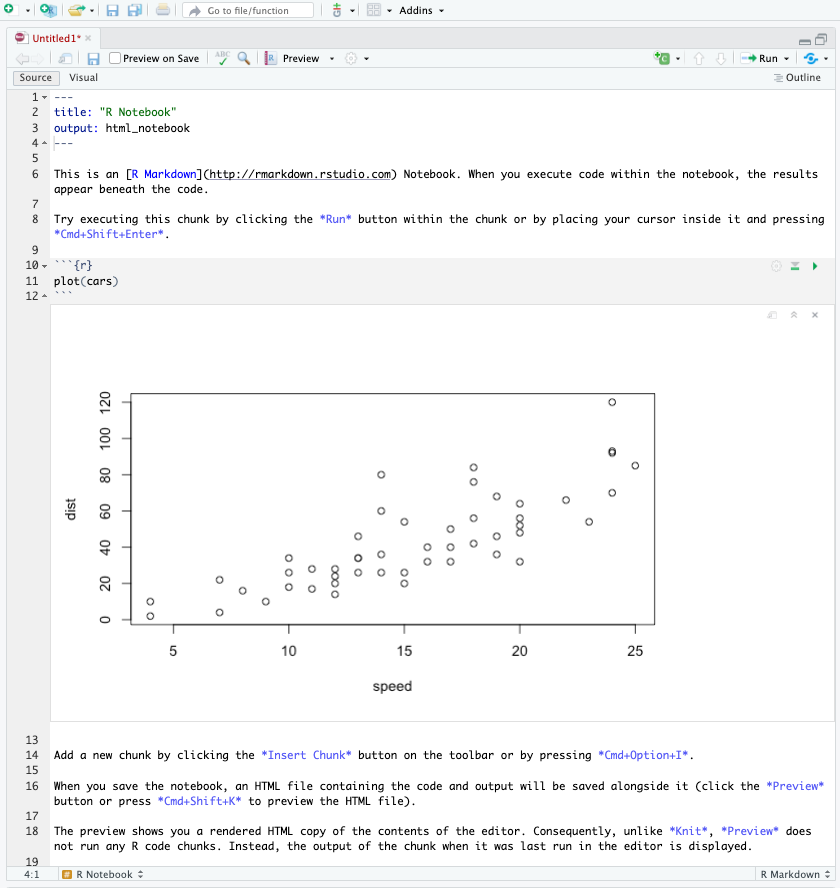
\includegraphics{images/R_notebook.png}

\hypertarget{section-2}{%
\subsection{}\label{section-2}}

\begin{Shaded}
\begin{Highlighting}[]
\FunctionTok{head}\NormalTok{(mpg, }\AttributeTok{n =} \DecValTok{3}\NormalTok{) }\SpecialCharTok{\%\textgreater{}\%}
  \FunctionTok{kbl}\NormalTok{() }\SpecialCharTok{\%\textgreater{}\%}
  \FunctionTok{kable\_styling}\NormalTok{()}
\end{Highlighting}
\end{Shaded}

\begin{table}
\centering
\begin{tabular}[t]{l|l|r|r|r|l|l|r|r|l|l}
\hline
manufacturer & model & displ & year & cyl & trans & drv & cty & hwy & fl & class\\
\hline
audi & a4 & 1.8 & 1999 & 4 & auto(l5) & f & 18 & 29 & p & compact\\
\hline
audi & a4 & 1.8 & 1999 & 4 & manual(m5) & f & 21 & 29 & p & compact\\
\hline
audi & a4 & 2.0 & 2008 & 4 & manual(m6) & f & 20 & 31 & p & compact\\
\hline
\end{tabular}
\end{table}

\hypertarget{ggplot2---themes}{%
\subsection{ggplot2 - Themes}\label{ggplot2---themes}}

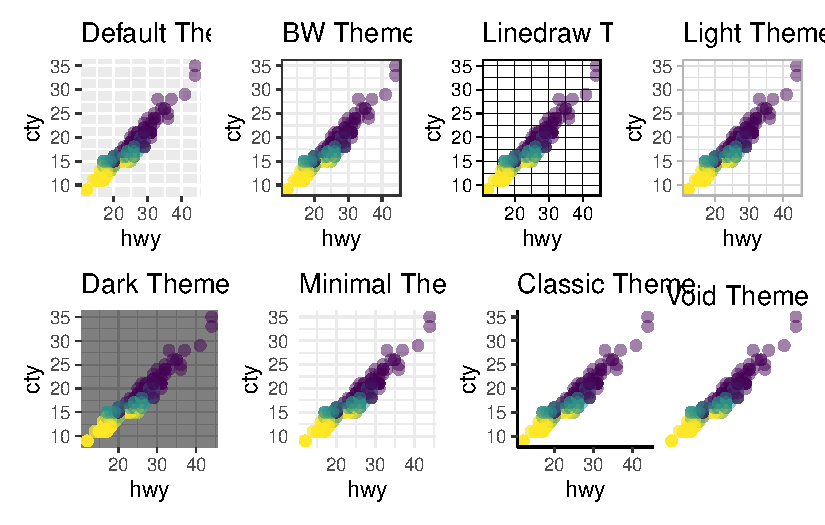
\includegraphics{RandRStudio_files/figure-pdf/unnamed-chunk-11-1.pdf}

\hypertarget{download-course-material}{%
\subsection{Download Course Material}\label{download-course-material}}

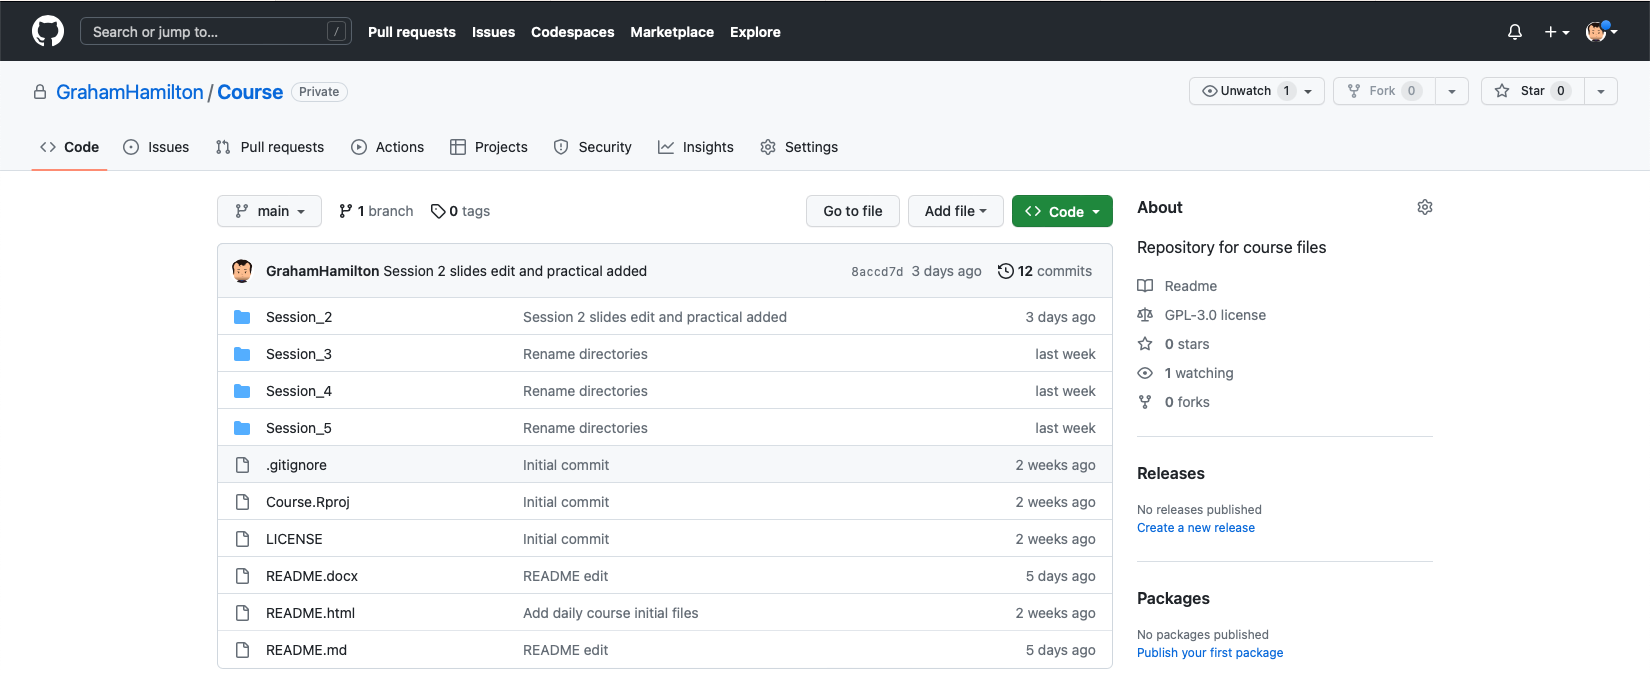
\includegraphics[width=\textwidth,height=5.20833in]{images/Github.png}

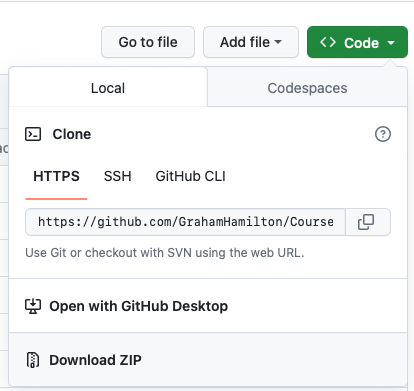
\includegraphics[width=\textwidth,height=3.125in]{images/Github_download.png}

\hypertarget{download-course-material-1}{%
\subsection{Download Course Material}\label{download-course-material-1}}

\begin{itemize}
\tightlist
\item
  Unzip the downloaded file
\item
  Move the folder to a suitable place on computer
\item
  Open RStudio and, using the files pane, navigate to the Course-main
  folder
\item
  Double click on the Course.Rproj
\end{itemize}

\hypertarget{ggplot2}{%
\subsection{ggplot2}\label{ggplot2}}

ggplot2 is a package for creating graphics

\begin{itemize}
\tightlist
\item
  Based on the Grammar of Graphics\\
\item
  Part of the tidyverse set of tools
\item
  Call ggplot()

  \begin{itemize}
  \tightlist
  \item
    Supply a suitably formatted data set\\
  \item
    What to plot from the data via aes (aesthetics), can also add
    colour, size, shape and transparency\\
  \item
    How the data is represented via the geom\_
  \end{itemize}
\end{itemize}

\hypertarget{ggplot2-1}{%
\subsection{ggplot2}\label{ggplot2-1}}

Set the data a plotting area, with ggplot and the aesthetics, to plot
the miles per gallon on the motorway on the x axis and miles per gallon
on the y axis

\begin{Shaded}
\begin{Highlighting}[]
\FunctionTok{ggplot}\NormalTok{(mpg, }\FunctionTok{aes}\NormalTok{(}\AttributeTok{x =}\NormalTok{ hwy, }\AttributeTok{y =}\NormalTok{ cty, }\AttributeTok{color =}\NormalTok{ cyl))}
\end{Highlighting}
\end{Shaded}

\begin{figure}[H]

{\centering 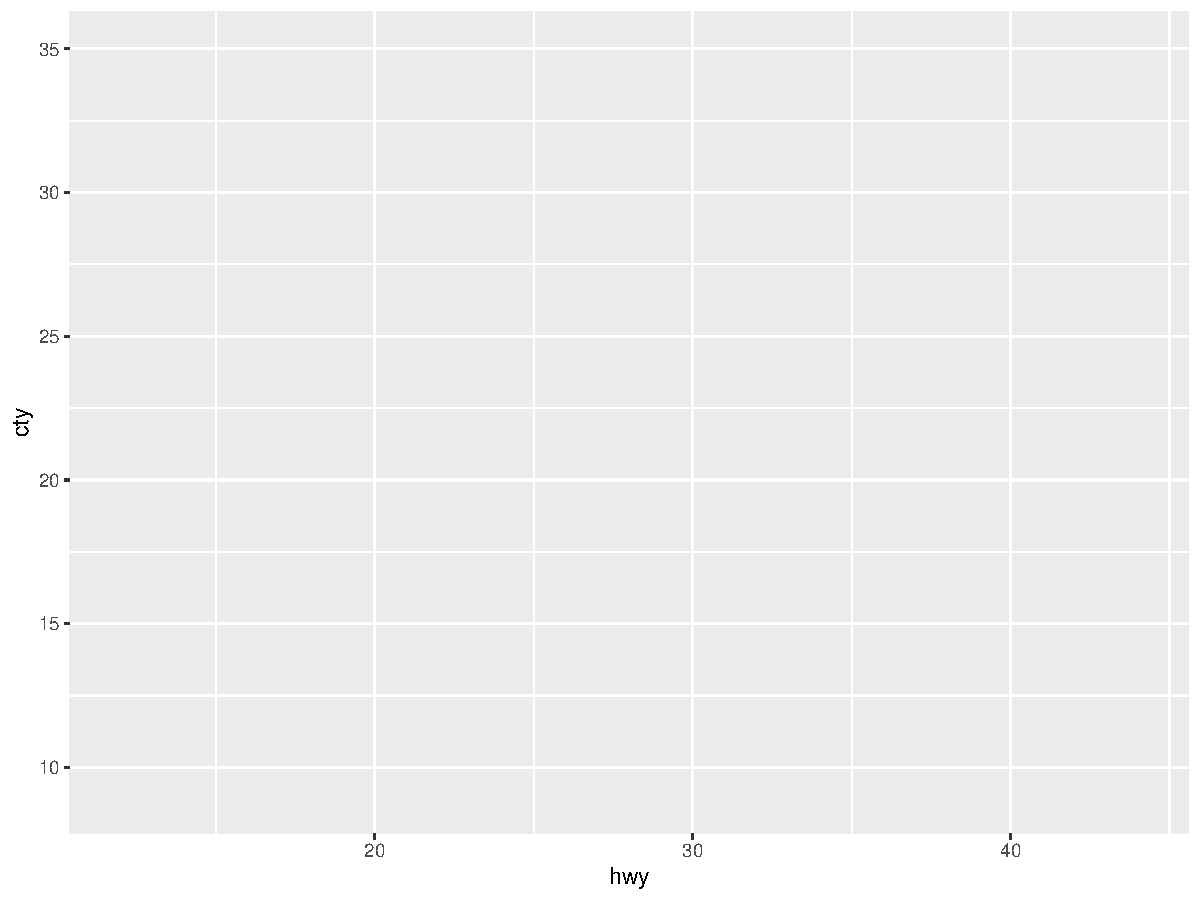
\includegraphics{RandRStudio_files/figure-pdf/unnamed-chunk-12-1.pdf}

}

\end{figure}

\hypertarget{ggplot2-2}{%
\subsection{ggplot2}\label{ggplot2-2}}

Scatter plot with geom\_point

\begin{Shaded}
\begin{Highlighting}[numbers=left,,]
\FunctionTok{ggplot}\NormalTok{(mpg, }\FunctionTok{aes}\NormalTok{(}\AttributeTok{x =}\NormalTok{ hwy, }\AttributeTok{y =}\NormalTok{ cty, }\AttributeTok{color =}\NormalTok{ cyl)) }\SpecialCharTok{+}
  \FunctionTok{geom\_point}\NormalTok{()}
\end{Highlighting}
\end{Shaded}

\begin{figure}[H]

{\centering 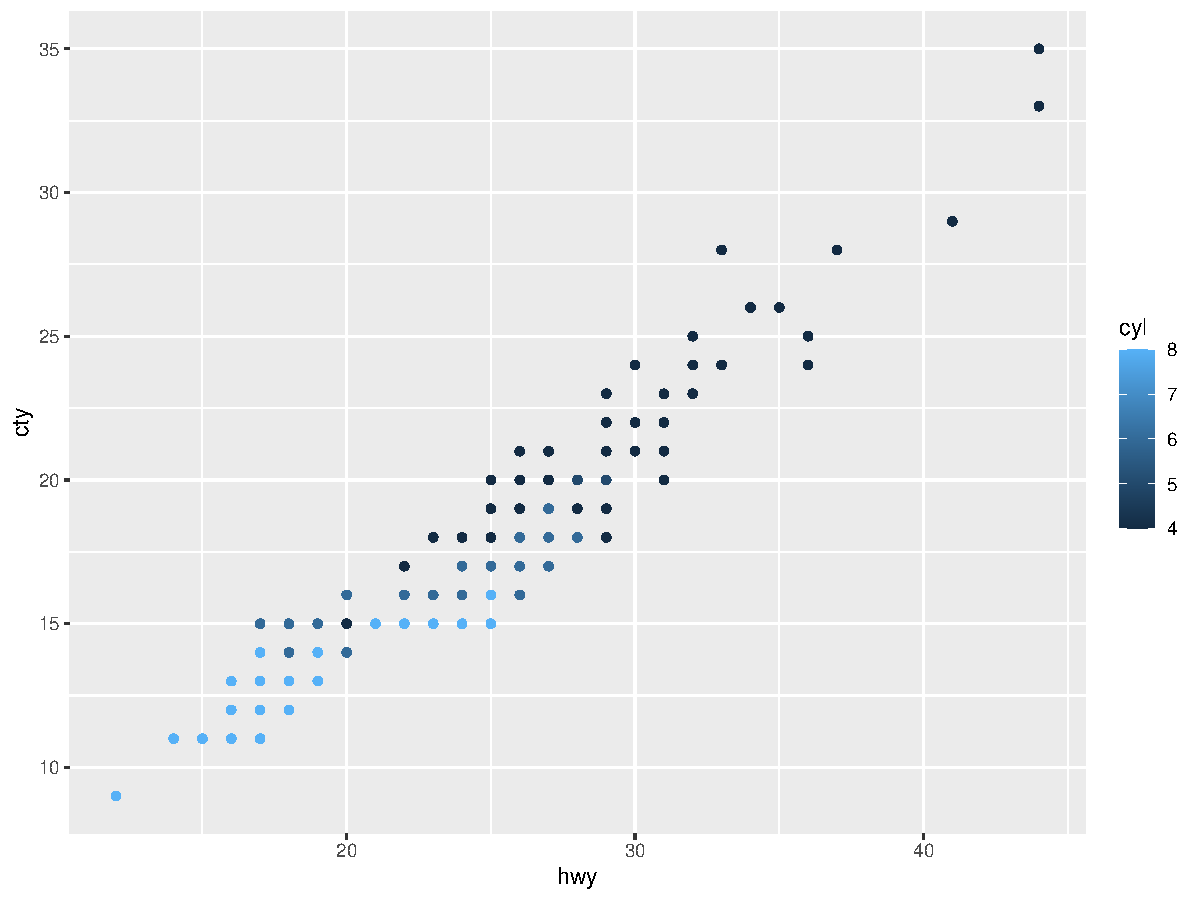
\includegraphics{RandRStudio_files/figure-pdf/unnamed-chunk-13-1.pdf}

}

\end{figure}

\hypertarget{ggplot2-3}{%
\subsection{ggplot2}\label{ggplot2-3}}

Change the transparency and size of the points

\begin{Shaded}
\begin{Highlighting}[numbers=left,,]
\FunctionTok{ggplot}\NormalTok{(mpg, }\FunctionTok{aes}\NormalTok{(}\AttributeTok{x =}\NormalTok{ hwy, }\AttributeTok{y =}\NormalTok{ cty, }\AttributeTok{color =}\NormalTok{ cyl)) }\SpecialCharTok{+}
  \FunctionTok{geom\_point}\NormalTok{(}\AttributeTok{alpha =} \FloatTok{0.5}\NormalTok{, }\AttributeTok{size =} \DecValTok{2}\NormalTok{)}
\end{Highlighting}
\end{Shaded}

\begin{figure}[H]

{\centering 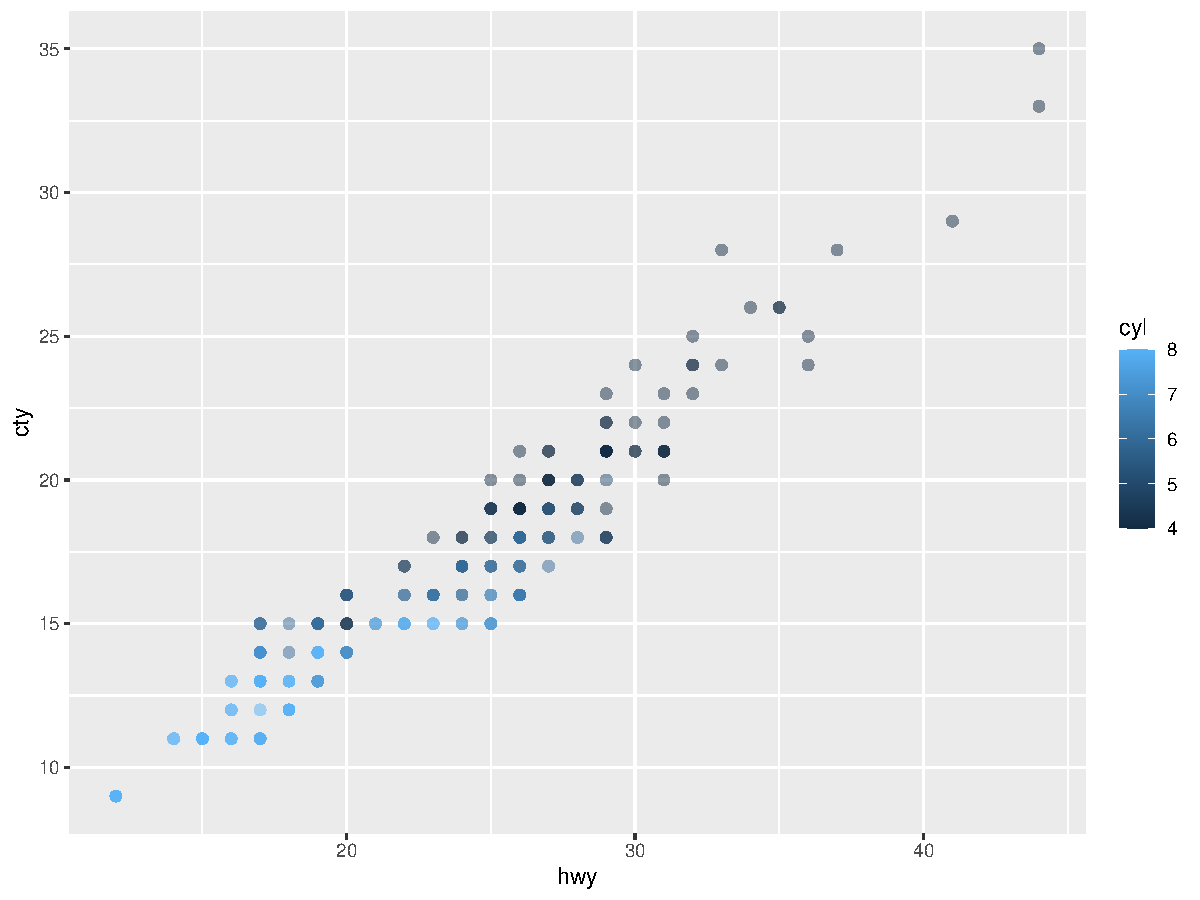
\includegraphics{RandRStudio_files/figure-pdf/unnamed-chunk-14-1.pdf}

}

\end{figure}

\hypertarget{ggplot2-4}{%
\subsection{ggplot2}\label{ggplot2-4}}

Change the point colours

\begin{Shaded}
\begin{Highlighting}[numbers=left,,]
\FunctionTok{ggplot}\NormalTok{(mpg, }\FunctionTok{aes}\NormalTok{(}\AttributeTok{x =}\NormalTok{ hwy, }\AttributeTok{y =}\NormalTok{ cty, }\AttributeTok{color =}\NormalTok{ cyl)) }\SpecialCharTok{+}
  \FunctionTok{geom\_point}\NormalTok{(}\AttributeTok{alpha =} \FloatTok{0.5}\NormalTok{, }\AttributeTok{size =} \DecValTok{2}\NormalTok{)  }\SpecialCharTok{+}
  \FunctionTok{scale\_color\_viridis\_c}\NormalTok{()}
\end{Highlighting}
\end{Shaded}

\begin{figure}[H]

{\centering 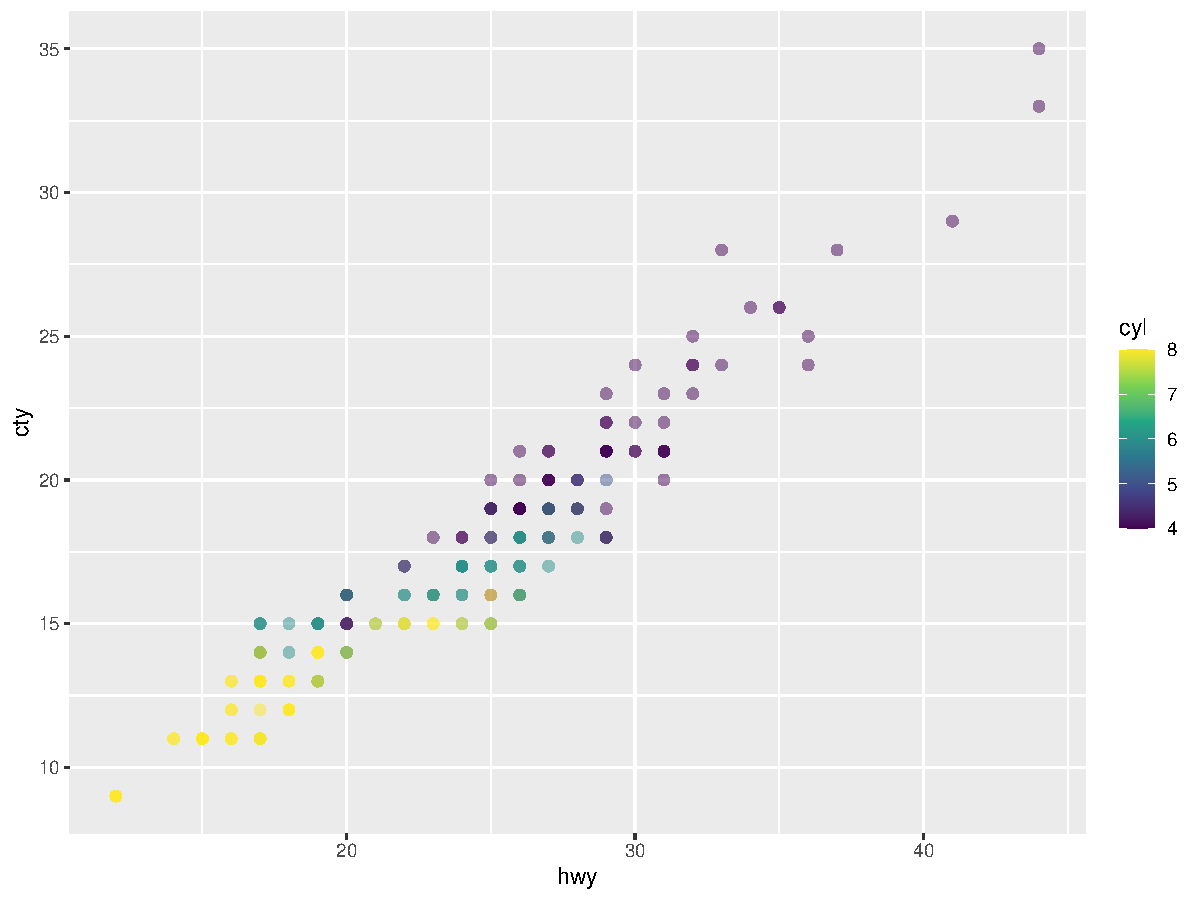
\includegraphics{RandRStudio_files/figure-pdf/unnamed-chunk-15-1.pdf}

}

\end{figure}

\hypertarget{ggplot2-5}{%
\subsection{ggplot2}\label{ggplot2-5}}

Add title and change axis labels

\begin{Shaded}
\begin{Highlighting}[numbers=left,,]
\FunctionTok{ggplot}\NormalTok{(mpg, }\FunctionTok{aes}\NormalTok{(}\AttributeTok{x =}\NormalTok{ hwy, }\AttributeTok{y =}\NormalTok{ cty, }\AttributeTok{color =}\NormalTok{ cyl)) }\SpecialCharTok{+}
  \FunctionTok{geom\_point}\NormalTok{(}\AttributeTok{alpha =} \FloatTok{0.5}\NormalTok{, }\AttributeTok{size =} \DecValTok{2}\NormalTok{)  }\SpecialCharTok{+}
  \FunctionTok{scale\_color\_viridis\_c}\NormalTok{() }\SpecialCharTok{+}
  \FunctionTok{labs}\NormalTok{(}\AttributeTok{title =} \StringTok{"Miles per gallon"}\NormalTok{,}
       \AttributeTok{x =} \StringTok{"Motorway miles per gallon"}\NormalTok{,}
       \AttributeTok{y =} \StringTok{"City miles per gallon"}\NormalTok{)}
\end{Highlighting}
\end{Shaded}

\begin{figure}[H]

{\centering 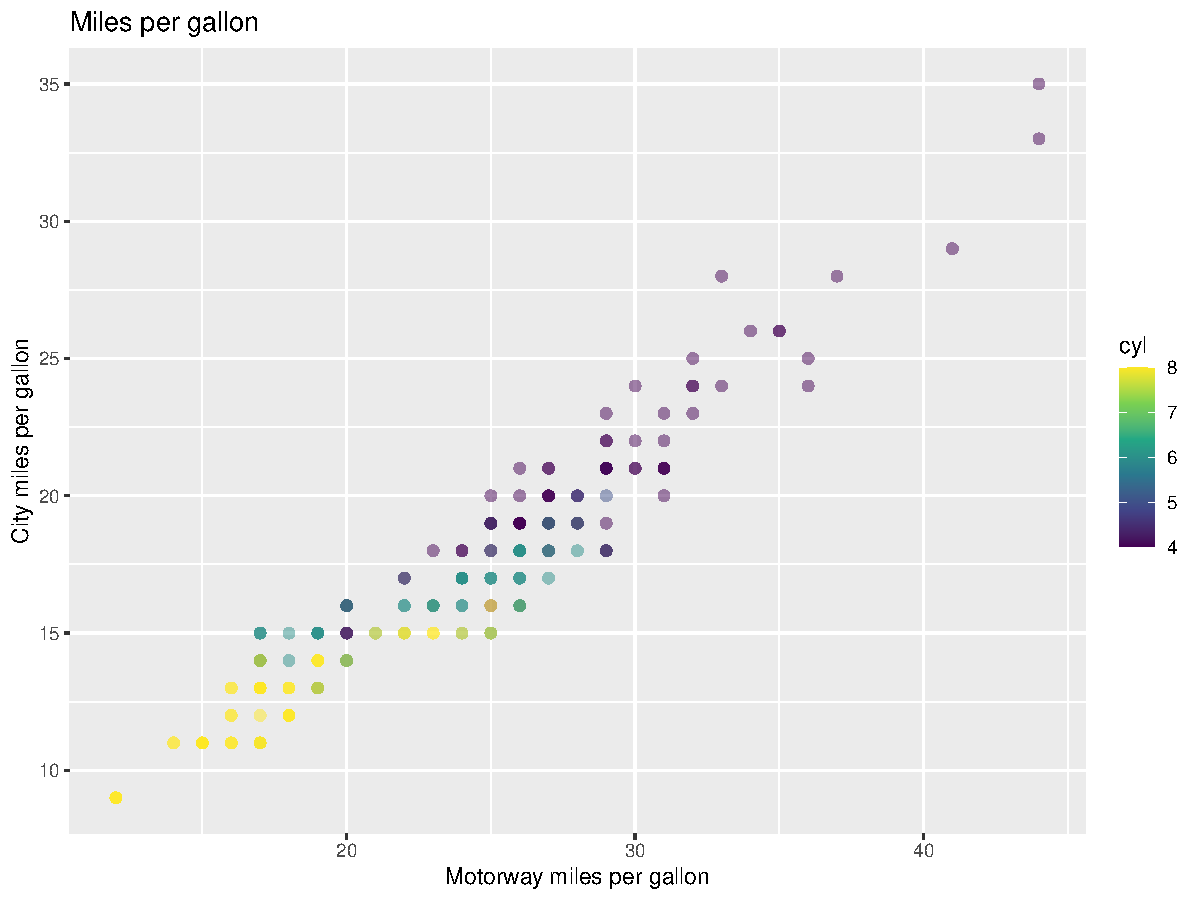
\includegraphics{RandRStudio_files/figure-pdf/unnamed-chunk-16-1.pdf}

}

\end{figure}

\hypertarget{ggplot2-6}{%
\subsection{ggplot2}\label{ggplot2-6}}

Box plot

\begin{Shaded}
\begin{Highlighting}[]
\NormalTok{mpg }\OtherTok{\textless{}{-}}\NormalTok{ mpg }\SpecialCharTok{\%\textgreater{}\%} \FunctionTok{mutate\_at}\NormalTok{(}\FunctionTok{vars}\NormalTok{(cyl), factor)}

\FunctionTok{ggplot}\NormalTok{(mpg, }\FunctionTok{aes}\NormalTok{(}\AttributeTok{x =}\NormalTok{ cyl, }\AttributeTok{y =}\NormalTok{ hwy, }\AttributeTok{fill =}\NormalTok{ cyl)) }\SpecialCharTok{+}
  \FunctionTok{geom\_boxplot}\NormalTok{() }\SpecialCharTok{+}
  \FunctionTok{scale\_fill\_viridis\_d}\NormalTok{()}
\end{Highlighting}
\end{Shaded}

\begin{figure}[H]

{\centering 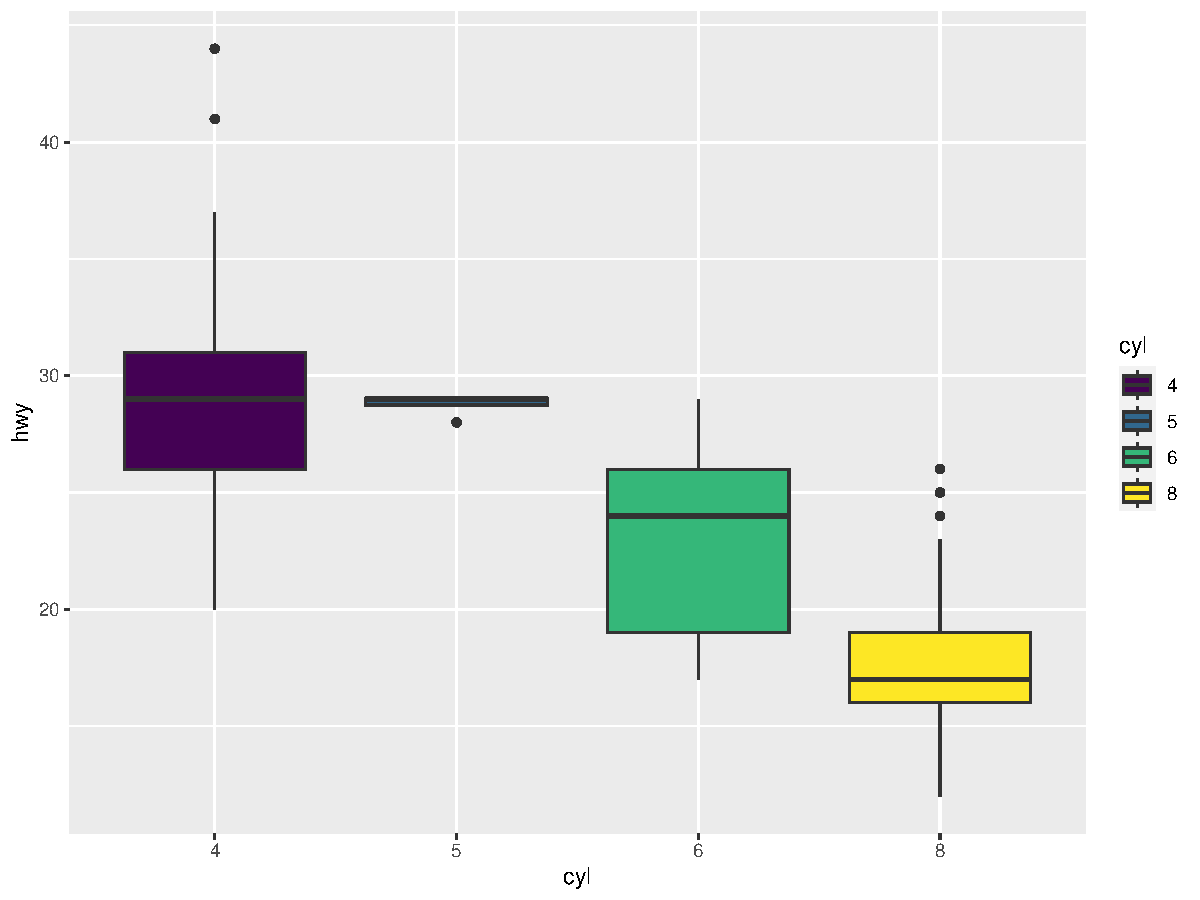
\includegraphics{RandRStudio_files/figure-pdf/unnamed-chunk-17-1.pdf}

}

\end{figure}

\hypertarget{ggplot2-7}{%
\subsection{ggplot2}\label{ggplot2-7}}

Box plot

\begin{Shaded}
\begin{Highlighting}[]
\NormalTok{mpg }\OtherTok{\textless{}{-}}\NormalTok{ mpg }\SpecialCharTok{\%\textgreater{}\%} \FunctionTok{mutate\_at}\NormalTok{(}\FunctionTok{vars}\NormalTok{(cyl), factor)}

\FunctionTok{ggplot}\NormalTok{(mpg, }\FunctionTok{aes}\NormalTok{(}\AttributeTok{x =}\NormalTok{ cyl, }\AttributeTok{y =}\NormalTok{ hwy, }\AttributeTok{fill =}\NormalTok{ cyl)) }\SpecialCharTok{+}
  \FunctionTok{geom\_boxplot}\NormalTok{() }\SpecialCharTok{+}
  \FunctionTok{geom\_jitter}\NormalTok{(}\AttributeTok{alpha =} \FloatTok{0.5}\NormalTok{, }\AttributeTok{size =} \DecValTok{2}\NormalTok{) }\SpecialCharTok{+}
  \FunctionTok{scale\_fill\_viridis\_d}\NormalTok{()}
\end{Highlighting}
\end{Shaded}

\begin{figure}[H]

{\centering 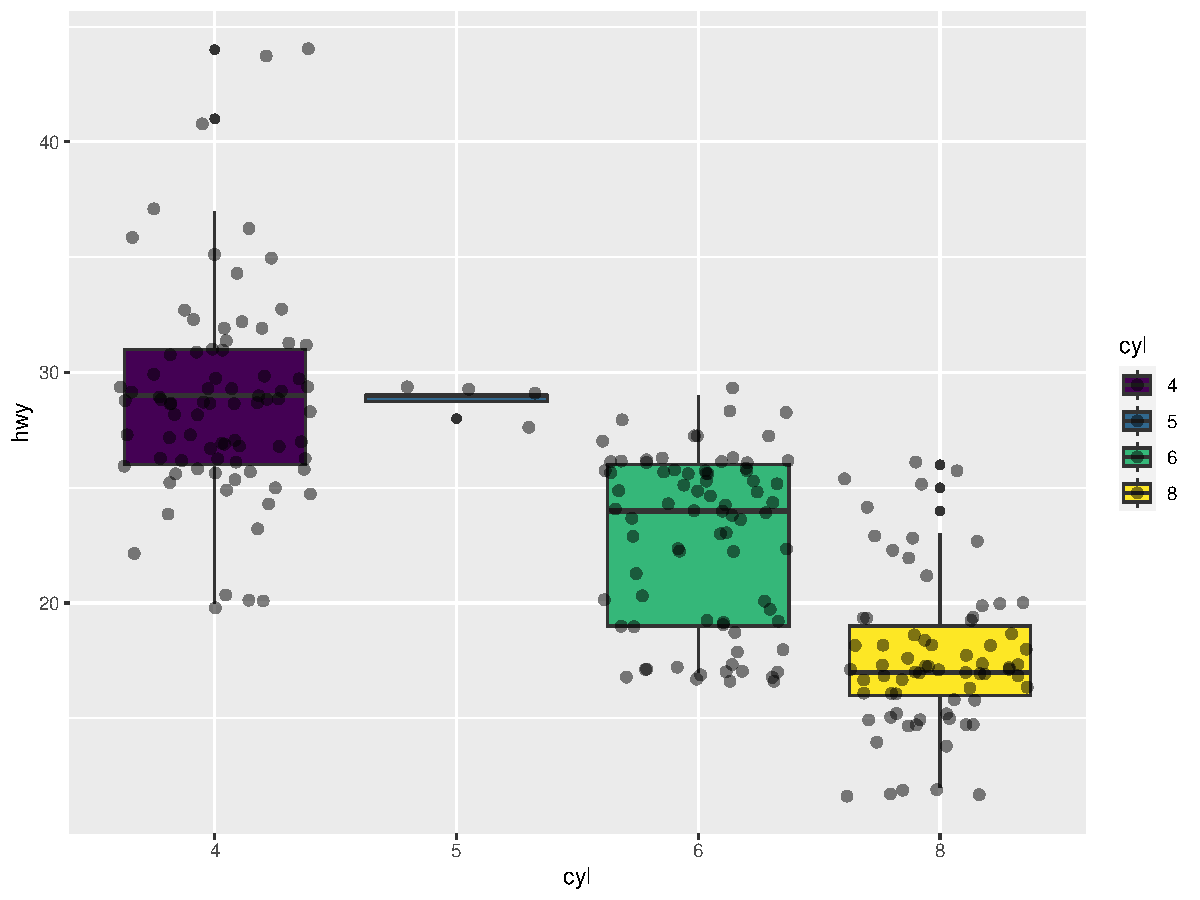
\includegraphics{RandRStudio_files/figure-pdf/unnamed-chunk-18-1.pdf}

}

\end{figure}

\hypertarget{ggplot2-8}{%
\subsection{ggplot2}\label{ggplot2-8}}

Violin plot

\begin{Shaded}
\begin{Highlighting}[]
\NormalTok{mpg }\OtherTok{\textless{}{-}}\NormalTok{ mpg }\SpecialCharTok{\%\textgreater{}\%} \FunctionTok{mutate\_at}\NormalTok{(}\FunctionTok{vars}\NormalTok{(cyl), factor)}

\FunctionTok{ggplot}\NormalTok{(mpg, }\FunctionTok{aes}\NormalTok{(}\AttributeTok{x =}\NormalTok{ cyl, }\AttributeTok{y =}\NormalTok{ hwy, }\AttributeTok{fill =}\NormalTok{ cyl)) }\SpecialCharTok{+}
  \FunctionTok{geom\_violin}\NormalTok{() }\SpecialCharTok{+}
  \FunctionTok{scale\_fill\_viridis\_d}\NormalTok{()}
\end{Highlighting}
\end{Shaded}

\begin{figure}[H]

{\centering 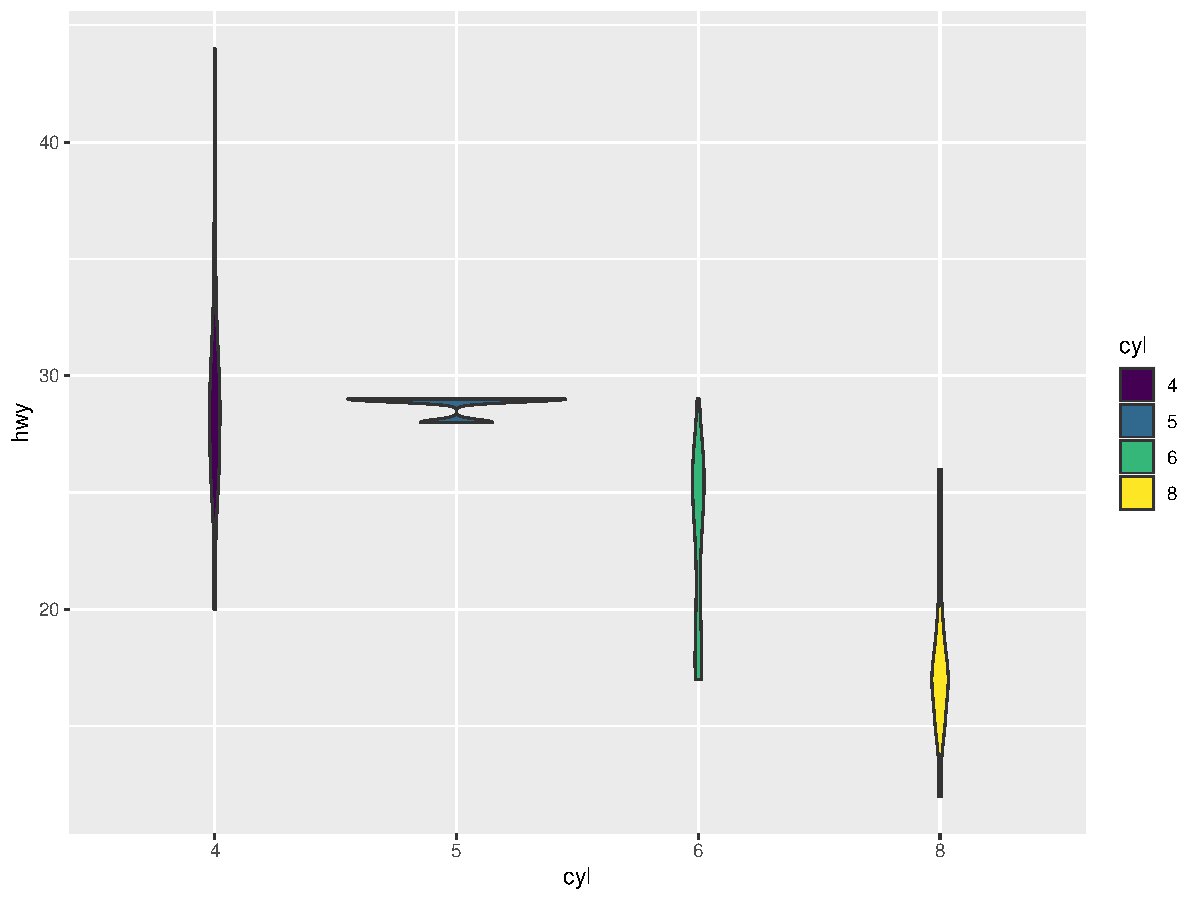
\includegraphics{RandRStudio_files/figure-pdf/unnamed-chunk-19-1.pdf}

}

\end{figure}

\hypertarget{tidyverse}{%
\subsection{Tidyverse}\label{tidyverse}}

\hypertarget{data-tidying}{%
\subsubsection{Data Tidying}\label{data-tidying}}

\begin{itemize}
\tightlist
\item
  First steps cleaning and preparing data
\item
  Time consuming
\item
  Packages supplied by the Tidyverse

  \begin{itemize}
  \item
    Share an underlying grammer and styructure
  \item
    Standardises data tidying
  \end{itemize}
\item
  Tidy data has:

  \begin{itemize}
  \tightlist
  \item
    Value, usually numbers
  \item
    Name, of a group to which the value belongs
  \end{itemize}
\end{itemize}

\hypertarget{tidyverse-1}{%
\subsection{Tidyverse}\label{tidyverse-1}}

The tidyverse is a collection of R packages designed for data science

\begin{itemize}
\item
  ggplot2
  
\includegraphics[width=1.04167in,height=\textheight]{images/ggplot2.png}

  \begin{itemize}
  \tightlist
  \item
    Package for creating graphics
  \end{itemize}
\item
  dplyr
  
\includegraphics[width=1.04167in,height=\textheight]{images/dplyr.png}

  \begin{itemize}
  \tightlist
  \item
    Package for data manipulation
  \end{itemize}
\end{itemize}

\begin{itemize}
\item
  tidyr
  
\includegraphics[width=1.04167in,height=\textheight]{images/tidyr.png}

  \begin{itemize}
  \tightlist
  \item
    Package for tidying data
  \end{itemize}
\item
  readr
  
\includegraphics[width=1.04167in,height=\textheight]{images/readr.png}

  \begin{itemize}
  \tightlist
  \item
    Package for reading in data
  \end{itemize}
\end{itemize}

https://www.tidyverse.org

\hypertarget{tidyverse-2}{%
\subsection{Tidyverse}\label{tidyverse-2}}

\begin{Shaded}
\begin{Highlighting}[]
\NormalTok{example\_table }\OtherTok{\textless{}{-}} \FunctionTok{read.table}\NormalTok{(}\StringTok{"data/example\_table.txt"}\NormalTok{, }\AttributeTok{header =} \ConstantTok{TRUE}\NormalTok{, }\AttributeTok{sep =} \StringTok{" "}\NormalTok{)}
\NormalTok{example\_table  }\SpecialCharTok{\%\textgreater{}\%}
  \FunctionTok{kbl}\NormalTok{() }\SpecialCharTok{\%\textgreater{}\%}
  \FunctionTok{kable\_styling}\NormalTok{()}
\end{Highlighting}
\end{Shaded}

\begin{table}
\centering
\begin{tabular}[t]{l|r|r}
\hline
Gene & Sample1 & Sample2\\
\hline
ACT1 & 100 & 120\\
\hline
NOTCH & 2 & 30\\
\hline
\end{tabular}
\end{table}

\begin{Shaded}
\begin{Highlighting}[]
\NormalTok{pivot\_table }\OtherTok{\textless{}{-}}\NormalTok{ example\_table }\SpecialCharTok{\%\textgreater{}\%} \FunctionTok{pivot\_longer}\NormalTok{(}\AttributeTok{cols =} \SpecialCharTok{{-}}\NormalTok{Gene, }\AttributeTok{names\_to =} \StringTok{"Sample"}\NormalTok{, }\AttributeTok{values\_to =} \StringTok{"Expression"}\NormalTok{)}
\NormalTok{pivot\_table }\SpecialCharTok{\%\textgreater{}\%}
  \FunctionTok{kbl}\NormalTok{() }\SpecialCharTok{\%\textgreater{}\%}
  \FunctionTok{kable\_styling}\NormalTok{()}
\end{Highlighting}
\end{Shaded}

\begin{table}
\centering
\begin{tabular}[t]{l|l|r}
\hline
Gene & Sample & Expression\\
\hline
ACT1 & Sample1 & 100\\
\hline
ACT1 & Sample2 & 120\\
\hline
NOTCH & Sample1 & 2\\
\hline
NOTCH & Sample2 & 30\\
\hline
\end{tabular}
\end{table}

\hypertarget{tidyverse-3}{%
\subsection{Tidyverse}\label{tidyverse-3}}

\begin{Shaded}
\begin{Highlighting}[]
\FunctionTok{ggplot}\NormalTok{(pivot\_table, }\FunctionTok{aes}\NormalTok{(}\AttributeTok{x =}\NormalTok{ Gene, }\AttributeTok{y =}\NormalTok{ Expression, }\AttributeTok{colour =}\NormalTok{ Gene)) }\SpecialCharTok{+}
  \FunctionTok{geom\_point}\NormalTok{(}\AttributeTok{size =} \DecValTok{5}\NormalTok{) }\SpecialCharTok{+}
  \FunctionTok{scale\_color\_viridis\_d}\NormalTok{()}
\end{Highlighting}
\end{Shaded}

\begin{figure}[H]

{\centering 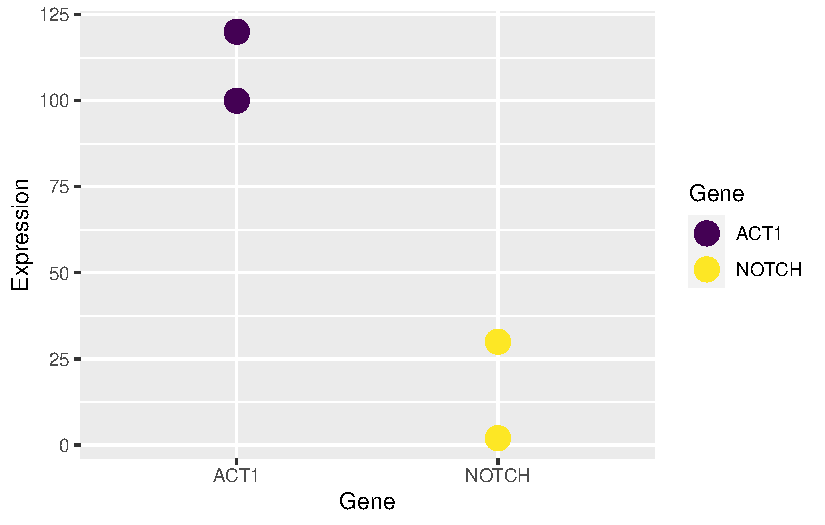
\includegraphics{RandRStudio_files/figure-pdf/unnamed-chunk-22-1.pdf}

}

\end{figure}

\newpage

\hypertarget{tidyverse-4}{%
\subsection{Tidyverse}\label{tidyverse-4}}

\begin{Shaded}
\begin{Highlighting}[]
\NormalTok{real\_data }\OtherTok{\textless{}{-}} \FunctionTok{read.table}\NormalTok{(}\StringTok{"data/real\_data\_example.tsv"}\NormalTok{, }\AttributeTok{header =} \ConstantTok{TRUE}\NormalTok{, }\AttributeTok{sep =} \StringTok{"}\SpecialCharTok{\textbackslash{}t}\StringTok{"}\NormalTok{)}
\FunctionTok{head}\NormalTok{(real\_data)  }\SpecialCharTok{\%\textgreater{}\%}
  \FunctionTok{kbl}\NormalTok{() }\SpecialCharTok{\%\textgreater{}\%}
  \FunctionTok{kable\_styling}\NormalTok{()}
\end{Highlighting}
\end{Shaded}

\begin{table}
\centering
\begin{tabular}[t]{l|r|r|r|r|r|r|r|r|r|r|r|r|r|r|r|r|r|r|r|r|r|r|r|r|r}
\hline
Gene\_names & Sample1\_1 & Sample1\_2 & Sample1\_3 & Sample1\_4 & Sample1\_5 & Sample2\_1 & Sample2\_2 & Sample2\_3 & Sample2\_4 & Sample2\_5 & Sample3\_1 & Sample3\_2 & Sample3\_3 & Sample3\_4 & Sample3\_5 & Sample4\_1 & Sample4\_2 & Sample4\_3 & Sample4\_4 & Sample4\_5 & Sample5\_1 & Sample5\_2 & Sample5\_3 & Sample5\_4 & Sample5\_5\\
\hline
CHAC1\_1279 & 49 & 11 & 0 & 254 & 11 & 30 & 61 & 18 & 0 & 34 & 26 & 47 & 0 & 0 & 21 & 23 & 50 & 102 & 0 & 71 & 0 & 67 & 11 & 1 & 59\\
\hline
GLRX\_2674 & 2212 & 1884 & 845 & 1262 & 1193 & 1868 & 1895 & 1378 & 1515 & 1964 & 1959 & 1602 & 1629 & 741 & 1145 & 310 & 538 & 185 & 332 & 705 & 358 & 526 & 278 & 157 & 1746\\
\hline
MEFV\_4116 & 214 & 278 & 47 & 115 & 0 & 120 & 20 & 23 & 824 & 52 & 121 & 150 & 129 & 20 & 66 & 26 & 55 & 98 & 53 & 100 & 10 & 20 & 31 & 66 & 80\\
\hline
STXBP1\_6866 & 361 & 283 & 196 & 362 & 163 & 221 & 333 & 183 & 109 & 203 & 131 & 150 & 187 & 149 & 352 & 100 & 122 & 129 & 150 & 163 & 0 & 233 & 26 & 83 & 69\\
\hline
AKAP8L\_196 & 203 & 34 & 86 & 101 & 0 & 149 & 56 & 254 & 168 & 41 & 83 & 61 & 174 & 62 & 42 & 88 & 107 & 66 & 113 & 209 & 103 & 49 & 168 & 100 & 114\\
\hline
AKR1C1\_199 & 18 & 22 & 0 & 279 & 235 & 0 & 51 & 0 & 54 & 0 & 145 & 66 & 52 & 3 & 52 & 14 & 54 & 0 & 83 & 0 & 85 & 0 & 22 & 27 & 18\\
\hline
\end{tabular}
\end{table}

\hypertarget{tidyverse-5}{%
\subsection{Tidyverse}\label{tidyverse-5}}

Tidy the data

\begin{Shaded}
\begin{Highlighting}[]
\NormalTok{pivot\_real\_data }\OtherTok{\textless{}{-}}\NormalTok{ real\_data }\SpecialCharTok{\%\textgreater{}\%} 
  \FunctionTok{pivot\_longer}\NormalTok{(}\SpecialCharTok{{-}}\NormalTok{Gene\_names, }\AttributeTok{names\_to =} \StringTok{"Samples"}\NormalTok{, }\AttributeTok{values\_to =} \StringTok{"Expression"}\NormalTok{)}

\FunctionTok{head}\NormalTok{(pivot\_real\_data)  }\SpecialCharTok{\%\textgreater{}\%}
  \FunctionTok{kbl}\NormalTok{() }\SpecialCharTok{\%\textgreater{}\%}
  \FunctionTok{kable\_styling}\NormalTok{()}
\end{Highlighting}
\end{Shaded}

\begin{table}
\centering
\begin{tabular}[t]{l|l|r}
\hline
Gene\_names & Samples & Expression\\
\hline
CHAC1\_1279 & Sample1\_1 & 49\\
\hline
CHAC1\_1279 & Sample1\_2 & 11\\
\hline
CHAC1\_1279 & Sample1\_3 & 0\\
\hline
CHAC1\_1279 & Sample1\_4 & 254\\
\hline
CHAC1\_1279 & Sample1\_5 & 11\\
\hline
CHAC1\_1279 & Sample2\_1 & 30\\
\hline
\end{tabular}
\end{table}

\hypertarget{tidyverse-6}{%
\subsection{Tidyverse}\label{tidyverse-6}}

Plot the data

\begin{Shaded}
\begin{Highlighting}[]
\FunctionTok{ggplot}\NormalTok{(pivot\_real\_data, }\FunctionTok{aes}\NormalTok{(}\AttributeTok{x =}\NormalTok{ Samples, }\AttributeTok{y =}\NormalTok{ Expression, }\AttributeTok{fill =}\NormalTok{ Samples)) }\SpecialCharTok{+}
  \FunctionTok{geom\_boxplot}\NormalTok{() }
\end{Highlighting}
\end{Shaded}

\begin{figure}[H]

{\centering 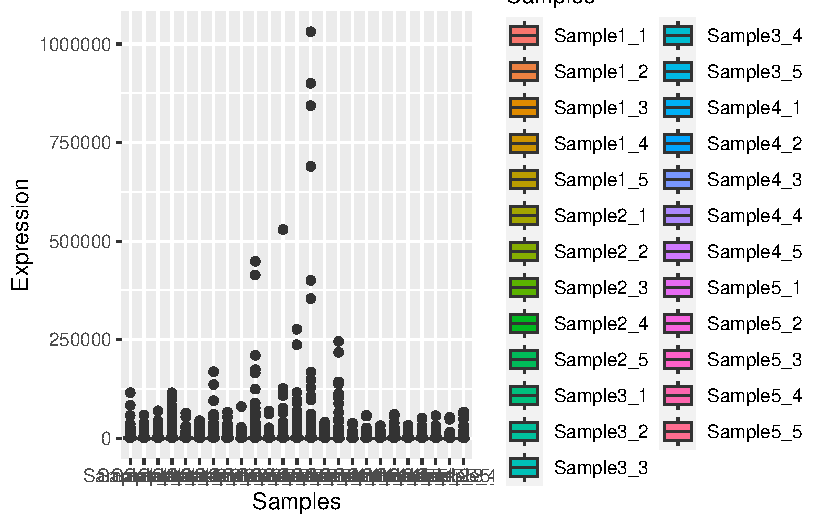
\includegraphics{RandRStudio_files/figure-pdf/unnamed-chunk-25-1.pdf}

}

\end{figure}

\hypertarget{tidyverse-7}{%
\subsection{Tidyverse}\label{tidyverse-7}}

Log transform the expression values

\begin{Shaded}
\begin{Highlighting}[numbers=left,,]
\FunctionTok{ggplot}\NormalTok{(pivot\_real\_data, }\FunctionTok{aes}\NormalTok{(}\AttributeTok{x =}\NormalTok{ Samples, }\AttributeTok{y =}\NormalTok{ Expression, }\AttributeTok{fill =}\NormalTok{ Samples)) }\SpecialCharTok{+}
  \FunctionTok{geom\_boxplot}\NormalTok{() }\SpecialCharTok{+}
  \FunctionTok{scale\_y\_log10}\NormalTok{() }
\end{Highlighting}
\end{Shaded}

\begin{verbatim}
Warning: Transformation introduced infinite values in continuous y-axis
\end{verbatim}

\begin{verbatim}
Warning: Removed 202816 rows containing non-finite values (`stat_boxplot()`).
\end{verbatim}

\begin{figure}[H]

{\centering 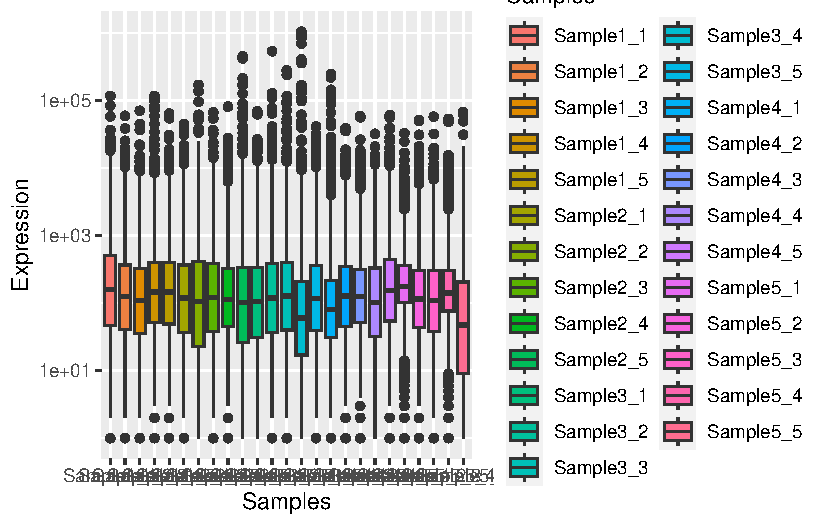
\includegraphics{RandRStudio_files/figure-pdf/unnamed-chunk-26-1.pdf}

}

\end{figure}

\hypertarget{tidyverse-8}{%
\subsection{Tidyverse}\label{tidyverse-8}}

Make the plot look prettier

\begin{Shaded}
\begin{Highlighting}[numbers=left,,]
\FunctionTok{ggplot}\NormalTok{(pivot\_real\_data, }\FunctionTok{aes}\NormalTok{(}\AttributeTok{x =}\NormalTok{ Samples, }\AttributeTok{y =}\NormalTok{ Expression, }\AttributeTok{fill =}\NormalTok{ Samples)) }\SpecialCharTok{+}
  \FunctionTok{geom\_boxplot}\NormalTok{() }\SpecialCharTok{+}
  \FunctionTok{scale\_y\_log10}\NormalTok{() }\SpecialCharTok{+}
  \FunctionTok{labs}\NormalTok{(}\AttributeTok{x =} \ConstantTok{NULL}\NormalTok{,}
       \AttributeTok{y =} \StringTok{"Log10(Expression)"}\NormalTok{) }\SpecialCharTok{+}
  \FunctionTok{scale\_fill\_viridis\_d}\NormalTok{() }\SpecialCharTok{+}
  \FunctionTok{theme\_classic}\NormalTok{() }\SpecialCharTok{+}
  \FunctionTok{theme}\NormalTok{(}\AttributeTok{legend.position =} \StringTok{"none"}\NormalTok{,}
        \AttributeTok{axis.text.x =} \FunctionTok{element\_text}\NormalTok{(}\AttributeTok{angle =} \DecValTok{90}\NormalTok{, }\AttributeTok{vjust =} \FloatTok{0.5}\NormalTok{, }\AttributeTok{hjust=}\DecValTok{1}\NormalTok{))}
\end{Highlighting}
\end{Shaded}

\begin{verbatim}
Warning: Transformation introduced infinite values in continuous y-axis
\end{verbatim}

\begin{verbatim}
Warning: Removed 202816 rows containing non-finite values (`stat_boxplot()`).
\end{verbatim}

\begin{figure}[H]

{\centering 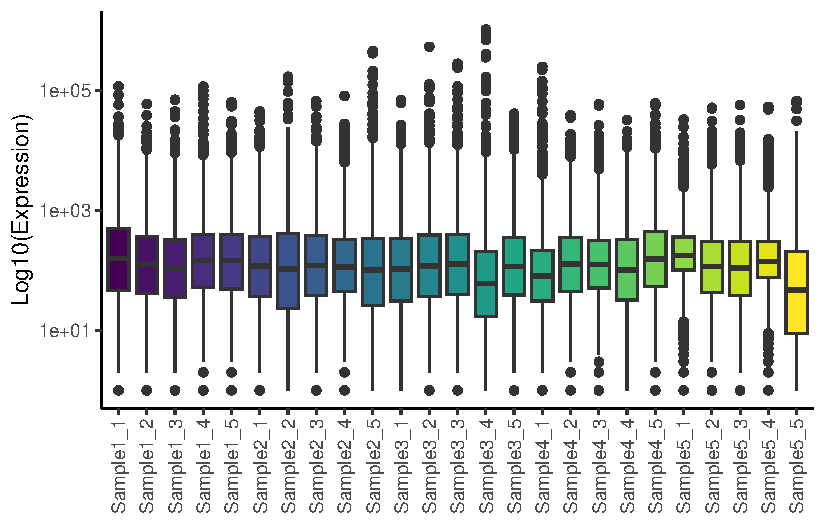
\includegraphics{RandRStudio_files/figure-pdf/unnamed-chunk-27-1.pdf}

}

\end{figure}

\hypertarget{tidyverse-9}{%
\subsection{Tidyverse}\label{tidyverse-9}}

Dplyr simplifies data manipulation

\begin{itemize}
\tightlist
\item
  Original table
\end{itemize}

\begin{Shaded}
\begin{Highlighting}[]
\FunctionTok{head}\NormalTok{(pivot\_table) }\SpecialCharTok{\%\textgreater{}\%}
  \FunctionTok{kbl}\NormalTok{() }\SpecialCharTok{\%\textgreater{}\%}
  \FunctionTok{kable\_styling}\NormalTok{()}
\end{Highlighting}
\end{Shaded}

\begin{table}
\centering
\begin{tabular}[t]{l|l|r}
\hline
Gene & Sample & Expression\\
\hline
ACT1 & Sample1 & 100\\
\hline
ACT1 & Sample2 & 120\\
\hline
NOTCH & Sample1 & 2\\
\hline
NOTCH & Sample2 & 30\\
\hline
\end{tabular}
\end{table}

\begin{itemize}
\tightlist
\item
  Select columns from a dataframe
\end{itemize}

\begin{Shaded}
\begin{Highlighting}[]
\NormalTok{pivot\_table }\SpecialCharTok{\%\textgreater{}\%}
  \FunctionTok{select}\NormalTok{(}\FunctionTok{c}\NormalTok{(Sample,Expression))}
\end{Highlighting}
\end{Shaded}

\begin{verbatim}
# A tibble: 4 x 2
  Sample  Expression
  <chr>        <int>
1 Sample1        100
2 Sample2        120
3 Sample1          2
4 Sample2         30
\end{verbatim}

\begin{itemize}
\tightlist
\item
  Filter rows that match a value in a column
\end{itemize}

\begin{Shaded}
\begin{Highlighting}[]
\NormalTok{pivot\_table }\SpecialCharTok{\%\textgreater{}\%}
  \FunctionTok{filter}\NormalTok{(Gene }\SpecialCharTok{==} \StringTok{"ACT1"}\NormalTok{)}
\end{Highlighting}
\end{Shaded}

\begin{verbatim}
# A tibble: 2 x 3
  Gene  Sample  Expression
  <chr> <chr>        <int>
1 ACT1  Sample1        100
2 ACT1  Sample2        120
\end{verbatim}

\hypertarget{section-3}{%
\subsection{}\label{section-3}}

\hypertarget{tidyverse-10}{%
\subsection{Tidyverse}\label{tidyverse-10}}

\begin{Shaded}
\begin{Highlighting}[]
\NormalTok{expression\_table }\OtherTok{\textless{}{-}}\NormalTok{ pivot\_real\_data }\SpecialCharTok{\%\textgreater{}\%}
  \FunctionTok{separate\_wider\_delim}\NormalTok{(Samples, }\AttributeTok{delim =} \StringTok{"\_"}\NormalTok{, }\AttributeTok{names =} \FunctionTok{c}\NormalTok{(}\StringTok{"Sample"}\NormalTok{, }\StringTok{"Replicate"}\NormalTok{)) }\SpecialCharTok{\%\textgreater{}\%}
  \FunctionTok{filter}\NormalTok{(Gene\_names }\SpecialCharTok{==} \StringTok{"CHAC1\_1279"}\NormalTok{)}
\end{Highlighting}
\end{Shaded}

\begin{Shaded}
\begin{Highlighting}[]
\FunctionTok{ggplot}\NormalTok{(expression\_table, }\FunctionTok{aes}\NormalTok{(}\AttributeTok{x =}\NormalTok{ Sample, }\AttributeTok{y =}\NormalTok{ Expression, }\AttributeTok{fill =}\NormalTok{ Sample)) }\SpecialCharTok{+}
  \FunctionTok{geom\_boxplot}\NormalTok{() }\SpecialCharTok{+}
  \FunctionTok{scale\_y\_log10}\NormalTok{() }\SpecialCharTok{+}
  \FunctionTok{labs}\NormalTok{(}\AttributeTok{x =} \ConstantTok{NULL}\NormalTok{,}
       \AttributeTok{y =} \StringTok{"Log10(Expression)"}\NormalTok{) }\SpecialCharTok{+}
  \FunctionTok{scale\_fill\_viridis\_d}\NormalTok{() }\SpecialCharTok{+}
  \FunctionTok{theme\_classic}\NormalTok{() }\SpecialCharTok{+}
  \FunctionTok{theme}\NormalTok{(}\AttributeTok{legend.position =} \StringTok{"none"}\NormalTok{)}
\end{Highlighting}
\end{Shaded}

\begin{verbatim}
Warning: Transformation introduced infinite values in continuous y-axis
\end{verbatim}

\begin{verbatim}
Warning: Removed 6 rows containing non-finite values (`stat_boxplot()`).
\end{verbatim}

\begin{figure}[H]

{\centering 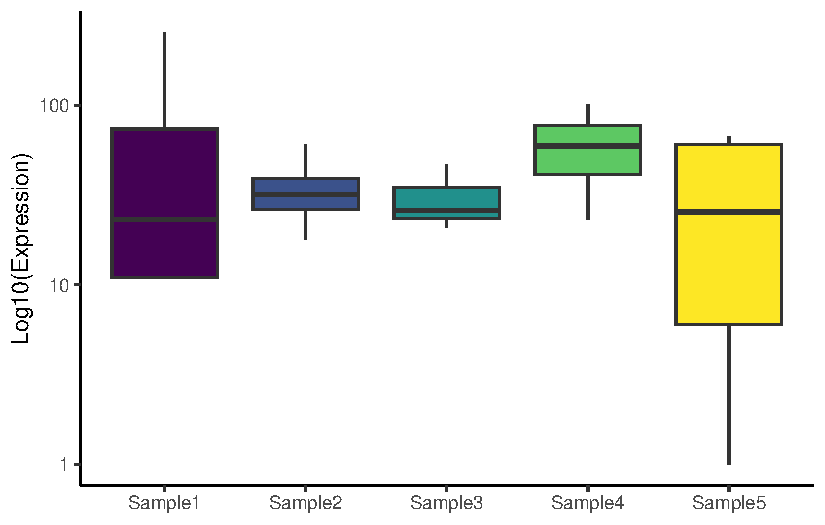
\includegraphics{RandRStudio_files/figure-pdf/unnamed-chunk-32-1.pdf}

}

\end{figure}



\end{document}
